\section{Experimentación y discusión}

  A continuación, se presentan las pruebas experimentales que se realizaron, junto con los resultados obtenidos y una discusión de los mismos. Estas pueden agruparse en dos grandes grupos: por un lado, aquellas llevadas a cabo con el fin de evaluar y comparar el rendimiento de los diferentes métodos ya presentados; por otra parte, las que se efectuaron para estudiar el comportamiento del sistema y los indicadores diseñados ante variaciones en los datos de entrada.

  Todos los experimentos se ejecutaron en las computadoras del laboratorio 4 del Departamento de Computación (\acr{FCEN - UBA}). 

  \subsection{Pruebas sobre el rendimiento de los métodos}

    \subsubsection{Experimento 1: Tiempo de ejecución según granularidad de la discretización} 

      \subsubsection*{Presentación}
        El objetivo de este experimento fue observar la relación entre los tiempos de ejecución y la granularidad de la discretización del dominio del problema, para los dos métodos implementados, manteniendo constantes los demás datos de entrada. 
        El experimento se realizó dos veces, uno para cada uno de los métodos numéricos. Manteniendo las temperaturas constantes, variamos cantidad de particiones de los ángulos dejando la de los radios intacta. Calculamos la solución del sistema para cada una de las distintas granularidades y comparamos los tiempos que toman las diferentes ejecuciones. Repetimos esto mismo, ahora variando las particiones de los radios. Luego tomamos el otro método numérico y volvemos a iniciar el experimento. 

      \subsubsection*{Datos de entrada}
        Para ambos casos, se construyeron escenarios de prueba con los siguientes parámetros: $r_i = 30$, $r_e = 60$, $T_i = 1500$, $c = 500$. La temperatura externa se consideró constante, con $T_e(\theta) = 50$ para todo $\theta$. En ambos casos las pruebas se realizaron utilizando primero el método de Eliminación Gaussiana y luego el de Factorización LU, y los tiempos de ejecución se tomaron en ciclos de reloj, utilizando las funciones provistas por la biblioteca estándar de \texttt{C++}. Para las pruebas se omitió realizar la estimación de la posición de la isoterma, limitándose a resolver el sistema por el método elegido ya que el cálculo de la isoterma es idéntico en ambos algoritmos y no afectará al análisis del tiempo de ejecución. 
      
        \begin{itemize}
          \item \strong{Caso A:} Se realizaron pruebas variando la cantidad de ángulos de la discretización, con $m + 1 = 30$ y $n = 10, 30, 50, 70, 90$. Se puede encontrar en los archivos adjuntos llamados \texttt{exp1a-\{n\}.in} la instancia pasada por parámetro.

          \item \strong{Caso B:} Se realizaron pruebas variando la cantidad de radios de la discretización, con $n = 60$ y $m+1 = 10, 30, 50, 70$. Se puede encontrar en los archivos adjuntos llamados \texttt{exp1b-\{m+1\}.in} la instancia pasada por parámetro.
        \end{itemize}

      \subsubsection*{Hipótesis}
        La complejidad del algoritmo es cúbico en el tamaño de la entrada. Como solo variamos la granularidad del radio o del ángulo (dejando el otro constante) entonces en ambos casos suponemos que el tiempo de ejecución va a ser cubico con relación a la granularidad de la entrada.

      \subsubsection*{Resultados}
       
        \begin{minipage}{\textwidth}
          \begin{center}
            \strong{Caso A}

            \begin{tabular}{cc}
              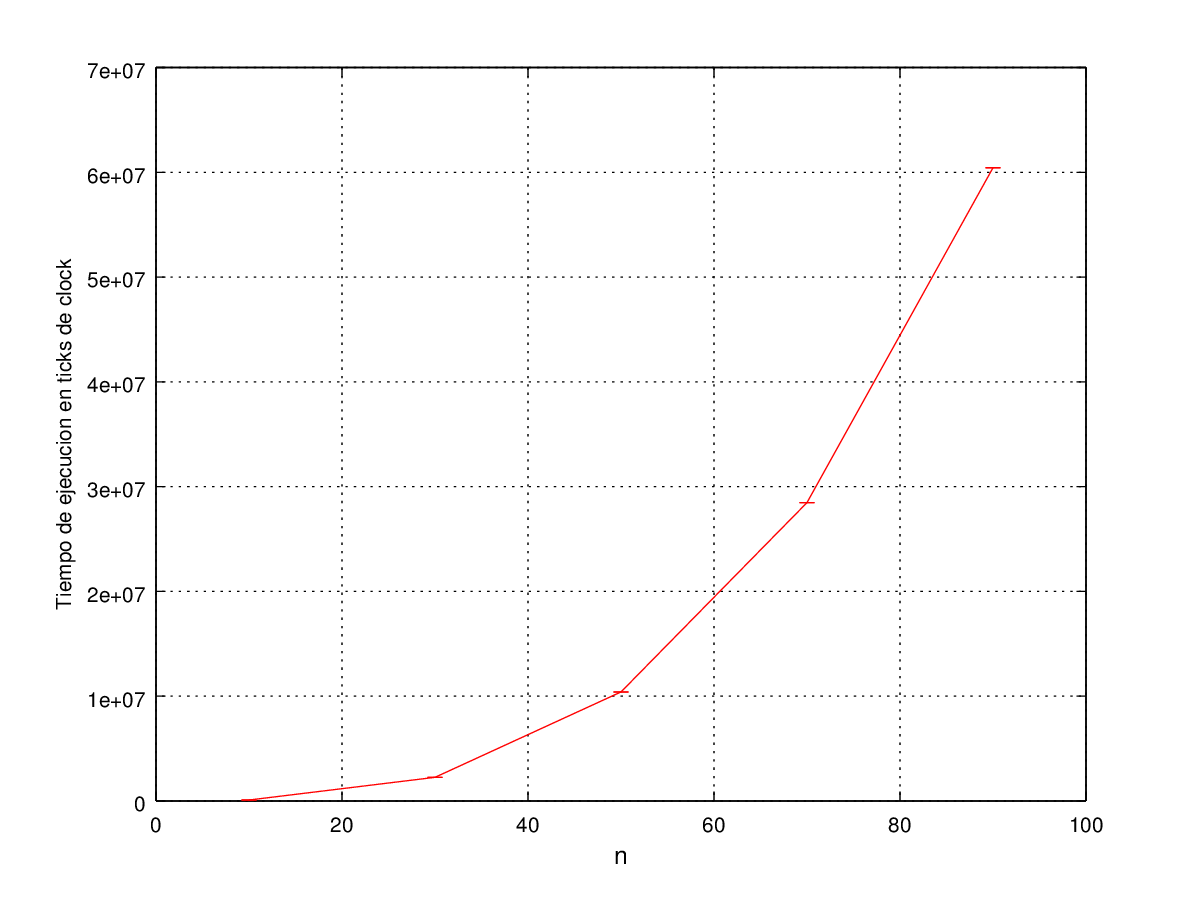
\includegraphics[width=8cm]{graficos/exp1/exp1-angulos0.png} & 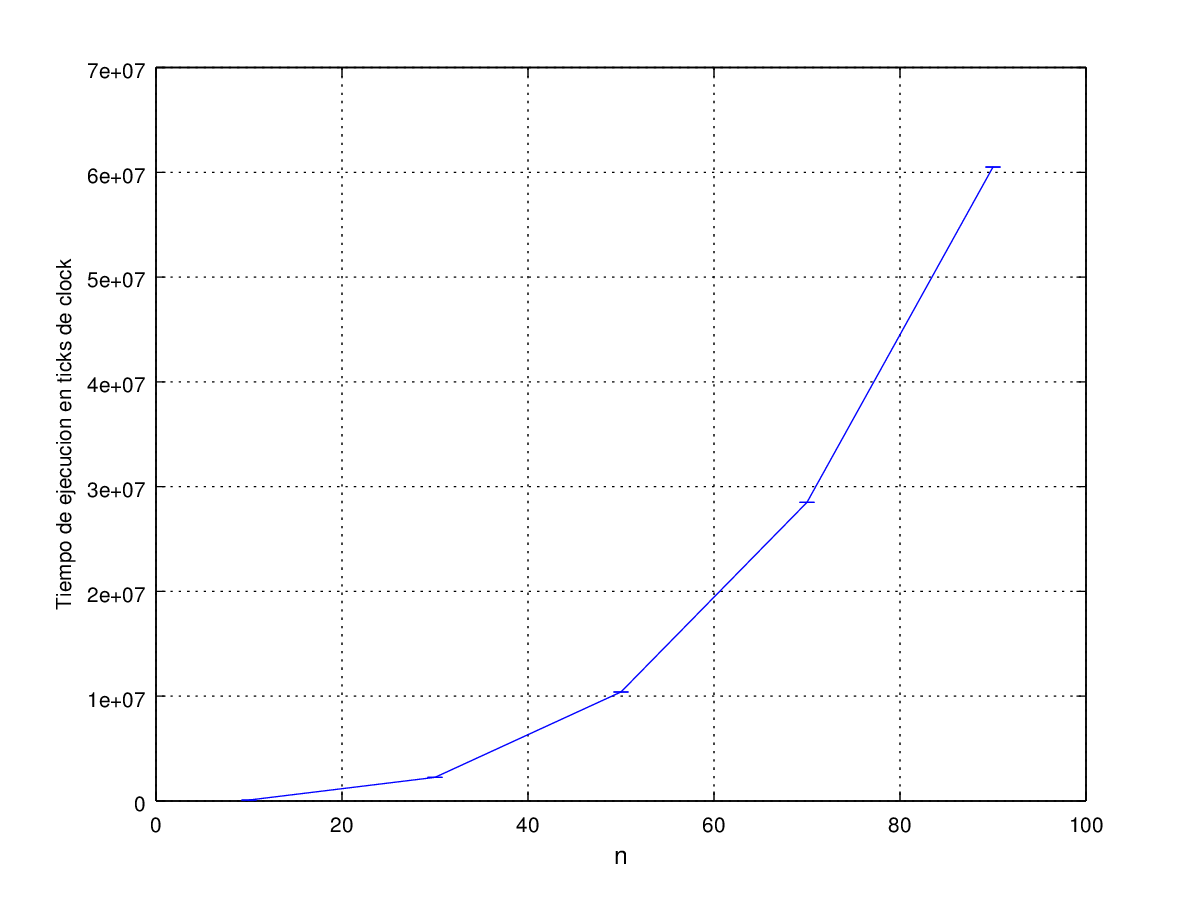
\includegraphics[width=8cm]{graficos/exp1/exp1-angulos1.png} \\
              {\small Eliminación Gaussiana} & {\small Factorización LU} \\
            \end{tabular}
          \end{center}
        \end{minipage}

        \vspace{1em}

        \begin{minipage}{\textwidth}
          \begin{center}
            \strong{Caso B}

            \begin{tabular}{cc}
              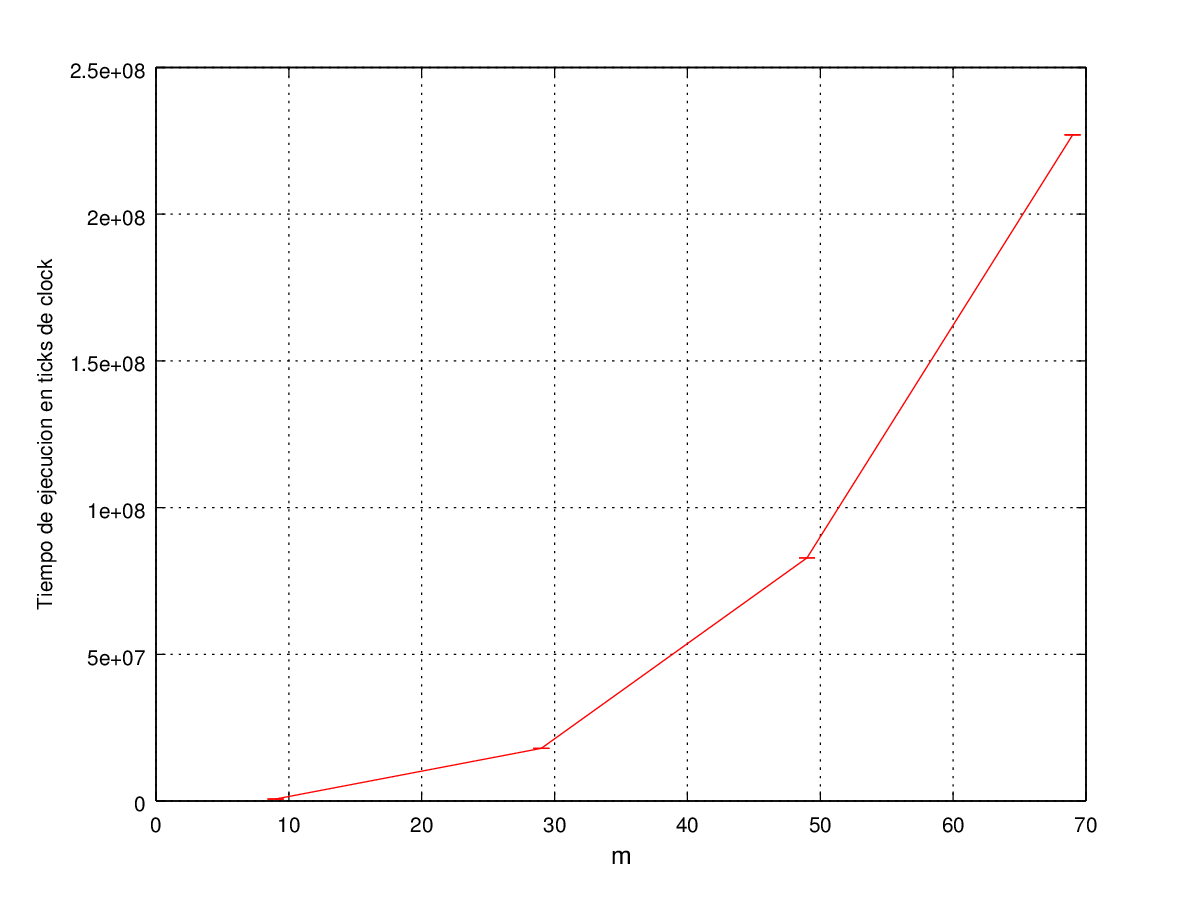
\includegraphics[width=8cm]{graficos/exp1/exp1-radios0.png} & 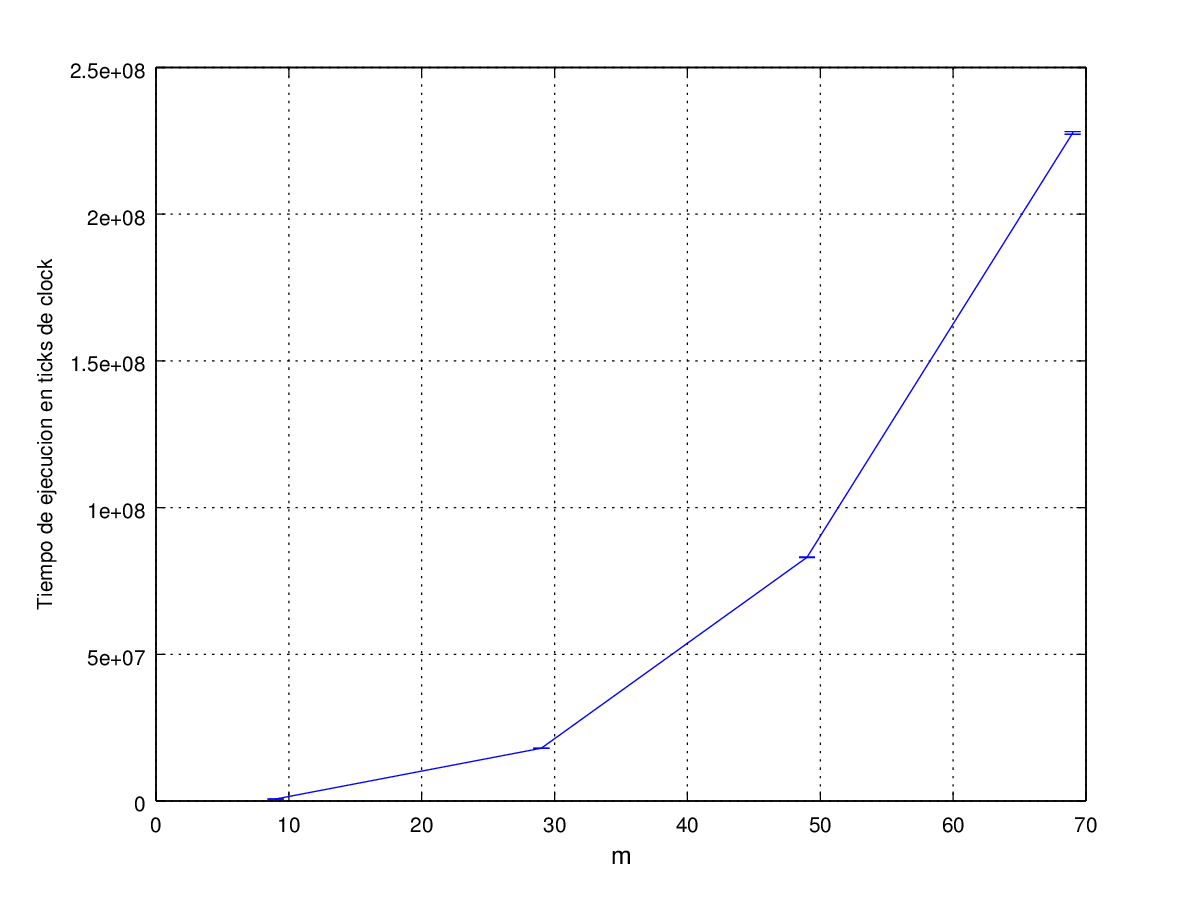
\includegraphics[width=8cm]{graficos/exp1/exp1-radios1.png} \\
              {\small Eliminación Gaussiana} & {\small Factorización LU} \\
            \end{tabular}

            \vspace{1em}
            {\small Resultados arrojados por el experimento 1}
          \end{center}
        \end{minipage}

      \subsubsection*{Discusión}
        En todos los gráficos correspondientes a este experimento, es claro el crecimiento del tiempo de ejecución a medida que la granularidad aumenta, tanto en los ángulos como en los radios. Esto se debe a la complejidad de los algoritmos utilizados. 
        Además, se puede observar que modificar la granularidad de radios o de ángulos es indistinto.

        También, es importante notar como el tiempo de ejecución sobre una sola instancia no cambia demasiado al modificar el método de resolución. Sabemos que, cuando se trata de un solo caso, factorización LU tiene complejidad mayor por constantes que eliminación gaussiana, lo que se puede visualizar en los casos con mayor granularidad de la discretización.

    \subsubsection{Experimento 2: Tiempo según número de instancias} 

      \subsubsection*{Presentación}
        En este experimento se generan distintas instancias para un mismo sistema, con el objetivo de comparar el tiempo de ejecución al resolverlas mediante el método de eliminación gaussiana y la factorización LU. 
        
        Para ello, se crean sistemas con diferentes cantidades de instancias y se comparan los tiempos de ejecución de los mismos para cada uno de los métodos. Con el fin de acercarse a los valores reales y descartar posibles falsos resultados, se ejecuta la resolución de un mismo sistema siete veces y se calcula el promedio de los tiempos medidos. 

      \subsubsection*{Datos}
        Se consideró una serie de 6 instancias del problema con los siguientes parámetros: $r_i = 10$, $r_e = 60$, $m+1 = 25$, $n = 40$, $T_i = 1500$, $c = 500$. Para las temperaturas externas se tomaron valores arbitrarios entre 50 y 200{\degree}C, diferentes en cada una de las instancias. Se puede encontrar en el archivo adjunto llamados \texttt{exp2-\{nInst\}.in} las instancias pasadas por parámetro.
  
        Se procesaron sucesivamente 1, 2, 3, 4, 5 y 6 instancias en corridas únicas del programa, utilizando primero el método de Eliminación Gaussiana y luego el de Factorización LU. Los tiempos de ejecución se tomaron en segundos, utilizando las funciones provistas por la biblioteca estándar de \texttt{C++}. Para las pruebas se omitió realizar la estimación de la posición de la isoterma, limitándose a resolver el sistema por el método elegido ya que el cálculo de la isoterma es idéntico en ambos algoritmos y no afectará al análisis del tiempo de ejecución. 

      \subsubsection*{Hipótesis}
        Conjeturamos que la diferencia entre los tiempos de ejecución de los dos métodos aumenta con la cantidad de instancias. 

        Al considerar un mismo sistema con diferentes instancias el método de eliminación gaussiana resulta más lento ya que resuelve cada una de ellas individualmente. En cambio, el método de factorización LU reutiliza la matriz $L$ ya calculada para resolver cada una de las instancias. 

        Destacamos que al considerar pocas instancias, factorización LU es más lenta que eliminación gaussiana, por una constante. Esto sucede ya que no se puede sacar ventaja de guardar la matriz $L$. 

      \subsubsection*{Resultados}
        
        \begin{minipage}{\textwidth} \begin{center}
          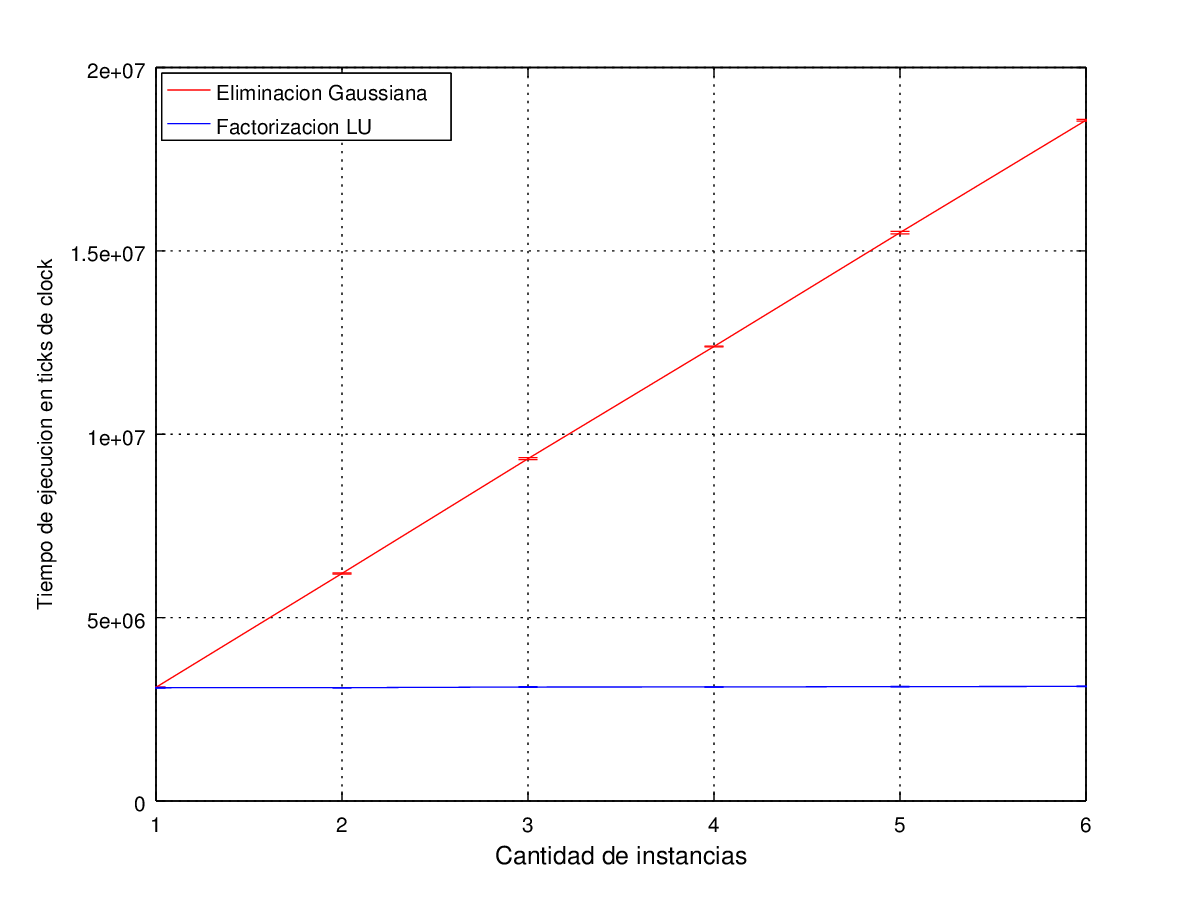
\includegraphics[width=11cm]{graficos/exp2/exp2.png}

          {\small Resultados arrojados por el experimento 2. Tiempo de ejecución en función del número de instancias del problema.}
        \end{center} \end{minipage}

      \subsubsection*{Discusión}
        Se observa que cuando hay pocas instancias, buscar la isoterma con el método de eliminación gaussiana o el de factorización LU es muy similar. 

        A medida que aumentan las instancias las diferencias entre ambos métodos aumentan, ya que la factorización LU se mantiene casi inmutable al aumentar las instancias mientras que la eliminación gaussiana aumenta notoriamente. 

        Se puede observar que lo que tarda la eliminación gaussiana cuando tiene 2 instancias es aproximadamente el doble de lo que tarda cuando es una única instancia. Cuando son 3 instancias, tarda el triple de lo que tarda cuando es una única instancia. 

        Sean $n$ instancias entonces lo que tarda la eliminación gaussiana es lo que tarda cuando es una única instancia $n$ veces. Esto es así ya que en este método numérico, para cada una de las instancias recalcula toda la matriz. En cambio la factorización LU, calcula la matriz una única vez.

  \subsection{Pruebas sobre el comportamiento del sistema}

    \subsubsection{Experimento 3: Isoterma según temperatura en pared externa} 
        
      \subsubsection*{Presentación}
        En este experimento vamos a observar como varía la isoterma cuando modificamos la temperatura de la pared externa del horno. Para ello tomamos dos sistemas con temperaturas externas constantes pero distintos entre sí. Graficamos para cada uno de ellos la isoterma 500. 
        
      \subsubsection*{Datos}
        Se evaluaron dos escenarios de prueba, ambos con los siguientes parámetros: $r_i = 30$, $r_e = 60$, $m+1 = 30$, $n = 30$, $T_i = 1500$, $c = 500$. Se utilizaron temperaturas externas constantes en todos los puntos $(r_e, \theta)$ de la discretización, con $T_e(\theta) = 50${\degree}C en uno de los casos y $T_e(\theta) = 200${\degree}C en el otro. Se puede encontrar en los archivos adjuntos llamados \texttt{exp3-\{T\textsubscript{e}($\theta$)\}.in} la instancia pasada por parámetro.

      \subsubsection*{Hipótesis}
        Suponemos que cuando mayor sea la temperatura, la isoterma estará mas cerca de la pared externa del alto horno. 

      \subsubsection*{Resultados}
        En el gráfico puede observarse la ubicación estimada de la isoterma para cada uno de los casos, en magenta para $T_e(\theta) = 50${\degree}C (Isoterma A) y en verde para $T_e(\theta) = 200${\degree}C (Isoterma B).
          
        \begin{minipage}{\textwidth} \begin{center}
          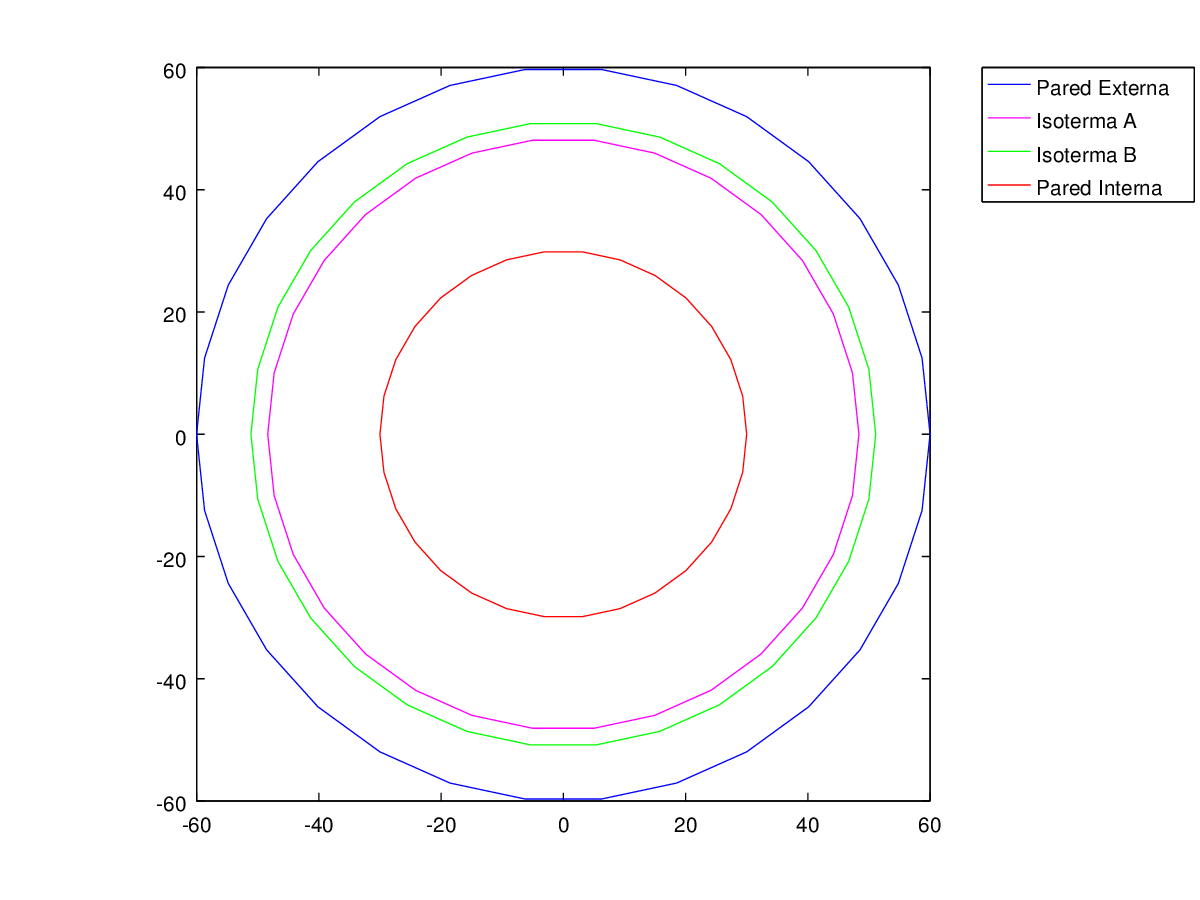
\includegraphics[width=11cm]{graficos/exp3/exp3.png} \\
          {\small Resultados arrojados por el experimento 3. Posiciones de las isotermas de 500{\degree}C.}
        \end{center} \end{minipage}

      \subsubsection*{Discusión}
        En este experimento se puede ver que la isoterma magenta se encuentra mas próxima a la pared interna del horno ya que corresponde a la instancia que tiene menor temperatura en la pared externa (50{\degree}C). La isoterma verde se encuentra más cerca de la pared externa debido a que las temperaturas son más altas (200{\degree}C).

        En uno de los casos la temperatura externa es la máxima posible y en el otro la mínima. Podemos observar que nunca, con esta discretización, para ningún valor de temperaturas externas válidas, la isoterma puede pasar mas cerca de la pared externa del alto horno que lo que pasa la isoterma marcada en el gráfico con verde. Tampoco es posible que la isoterma pase más cerca de la pared interna del horno de lo que pasa la isoterma marcada en el gráfico con color magenta.

    \subsubsection{Experimento 4: Isoterma según granularidad} 
        
      \subsubsection*{Presentación}
        Para realizar este experimento, se calcula la isoterma en un sistema donde la temperatura de la pared externa es constante, y la granularidad es muy alta. Llamaremos a esta, la isoterma de contraste. Se planea observar como varía la isoterma cuando se disminuye esta granularidad modificando únicamente la cantidad de radios a tener en cuenta (sin cambiar los ángulos), o modificando la cantidad de ángulos (sin cambiar los radios).
        Luego, se repite este proceso pero variando los valores de las temperaturas de la pared externa del horno. Esto valores son generados utilizando la función seno.

      \subsubsection*{Datos}

        \begin{enumerate}[label=(\roman*)]
          \item \strong{Temperaturas constantes}

            Para ambos casos se consideraron instancias de prueba con los siguientes parámetros: $r_i = 30$, $r_e = 60$, $T_i = 1500$, $c = 500$. Se utilizó una temperatura externa constante en todos los puntos $(r_e, \theta)$ de la discretización, ($T_e(\theta) = 50$). 

            En primer lugar, se calculó la solución del sistema y la posición estimada de la isoterma para una discretización considerablemente granular, con $m + 1 = 70$ y $n = 90$, para utilizar como caso de contraste. 

            \begin{itemize}
              \item \strong{Caso A:} Se mantuvo constante la cantidad de radios de la discretización $m + 1 = 70$, y se tomaron instancias con diferentes cantidades de ángulos, para $n = 3, 5, 8, 10, 30, 50, 70$. Los gráficos que incluimos representan los resultados obtenidos para $n = 5, 10, 50$, reflejando las temperaturas calculadas y la ubicación estimada de la isoterma (en verde), comparada con la obtenida para el caso de contraste (en magenta). Se puede encontrar en los archivos adjuntos llamados \texttt{exp4-const-ang-\{n\}.in} la instancia pasada por parámetro.

              \item \strong{Caso B:} Se mantuvo constante la cantidad de ángulos de la discretización $n = 90$, y se tomaron instancias con diferentes cantidades de radios, para $m + 1 = 3, 5, 8, 10, 30, 50$. Los gráficos que incluimos representan los resultados obtenidos para $m + 1 = 3, 8, 30$, reflejando las temperaturas calculadas y la ubicación estimada de la isoterma (en verde), comparada con la obtenida para el caso de contraste (en magenta). Se puede encontrar en los archivos adjuntos llamados \texttt{exp4-const-rad-\{m+1\}.in} la instancia pasada por parámetro.
            \end{itemize}

          \item \strong{Temperaturas variables}

            Para ambos casos se consideraron instancias de prueba con los siguientes parámetros: $r_i = 30$, $r_e = 60$, $T_i = 1500$, $c = 500$. Se generó una instancia de prueba con una temperatura externa variable entre 50 y 200{\degree}C en todos los puntos $(r_e, \theta)$ de la discretización. 
            Para la generación de las instancias de prueba se consideró la función $T_e(\theta) = 125 + 75 \sin(2\theta)$ para que la variación de temperaturas sea suave.
            En primer lugar, se calculó la solución del sistema y la posición estimada de la isoterma para una discretización considerablemente granular, con $m + 1 = 70$ y $n = 90$, para utilizar como caso de contraste. Reproducimos los gráficos que representan las temperaturas calculadas para todos los puntos de la discretización y la ubicación estimada de la isoterma.

            \begin{itemize}
              \item \strong{Caso A:} Se mantuvo constante la cantidad de radios de la discretización $m + 1 = 70$, y se tomaron instancias con diferentes cantidades de ángulos, para $n = 3, 5, 8, 10, 30, 50, 70$. Los gráficos que incluimos representan los resultados obtenidos para $n = 5, 10, 50$, reflejando las temperaturas calculadas y la ubicación estimada de la isoterma (en verde), comparada con la obtenida para el caso de contraste (en magenta). Se puede encontrar en los archivos adjuntos llamados \texttt{exp4-seno-ang-\{n\}.in} la instancia pasada por parámetro.
            
              \item \strong{Caso B:} Se mantuvo constante la cantidad de ángulos de la discretización $n = 90$, y se tomaron instancias con diferentes cantidades de ángulos, para $m + 1 = 3, 5, 8, 10, 30, 50$. Los gráficos que incluimos representan los resultados obtenidos para $m + 1 = 3, 8, 30$, reflejando las temperaturas calculadas y la ubicación estimada de la isoterma (en verde), comparada con la obtenida para el caso de contraste (en magenta). Se puede encontrar en los archivos adjuntos llamados \texttt{exp4-seno-rad-\{m+1\}.in} la instancia pasada por parámetro.
            \end{itemize}

        \end{enumerate}
     
      \subsubsection*{Hipótesis}
        Se espera que, en ambos casos, cuanto menor sea la granularidad de la discretización, más alejada estará la isoterma calculada de la de contraste. Si tomamos menos particiones sobre radios, la distancia entre ellos aumenta. Como el cálculo de la isoterma supone que la temperatura entre dos de ellos, uno más lejano y otro más cercano a la pared, decrece en forma lineal, lo cual podría generar que el error aumente. Si se toman menos particiones sobre ángulos, existen puntos que no van a ser considerados en el cálculo de la isoterma, por lo tanto, el error también es mayor. 

      \subsubsection*{Resultados}
        Para estos gráficos se tomará el color rojo como las temperaturas más calientes siendo el rojo más oscuro la temperatura de 1500{\degree}C y azul las temperaturas más frías siendo el azul más oscuro 50{\degree}C.

        \begin{minipage}{\textwidth}
                
        (\textsc{i}) \strong{Temperaturas constantes}

        \begin{center}

          \strong{Caso de contraste} ($m + 1 = 70$ y $n = 90$)

          \begin{tabular}{cc}
            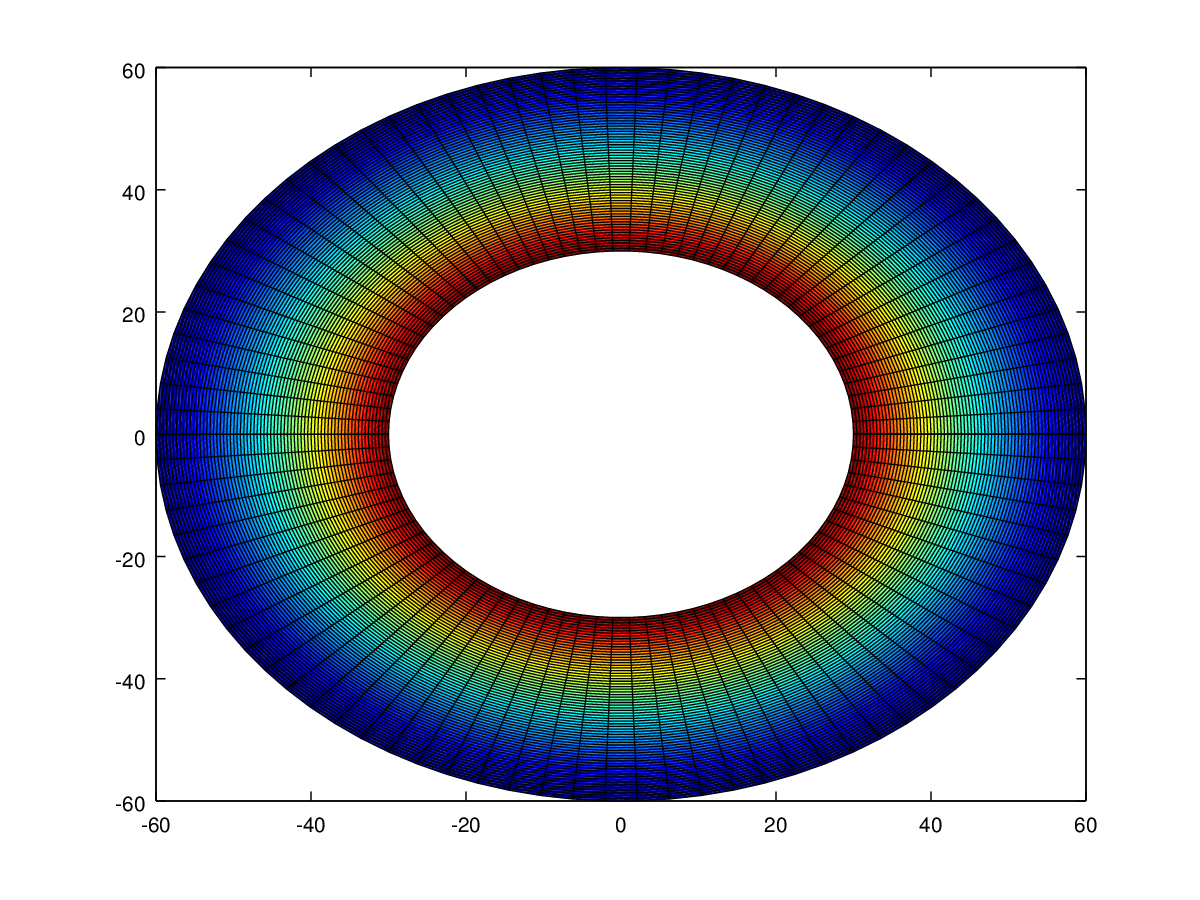
\includegraphics[height=5cm]{graficos/exp4/const/exp4-const-contraste.png} & 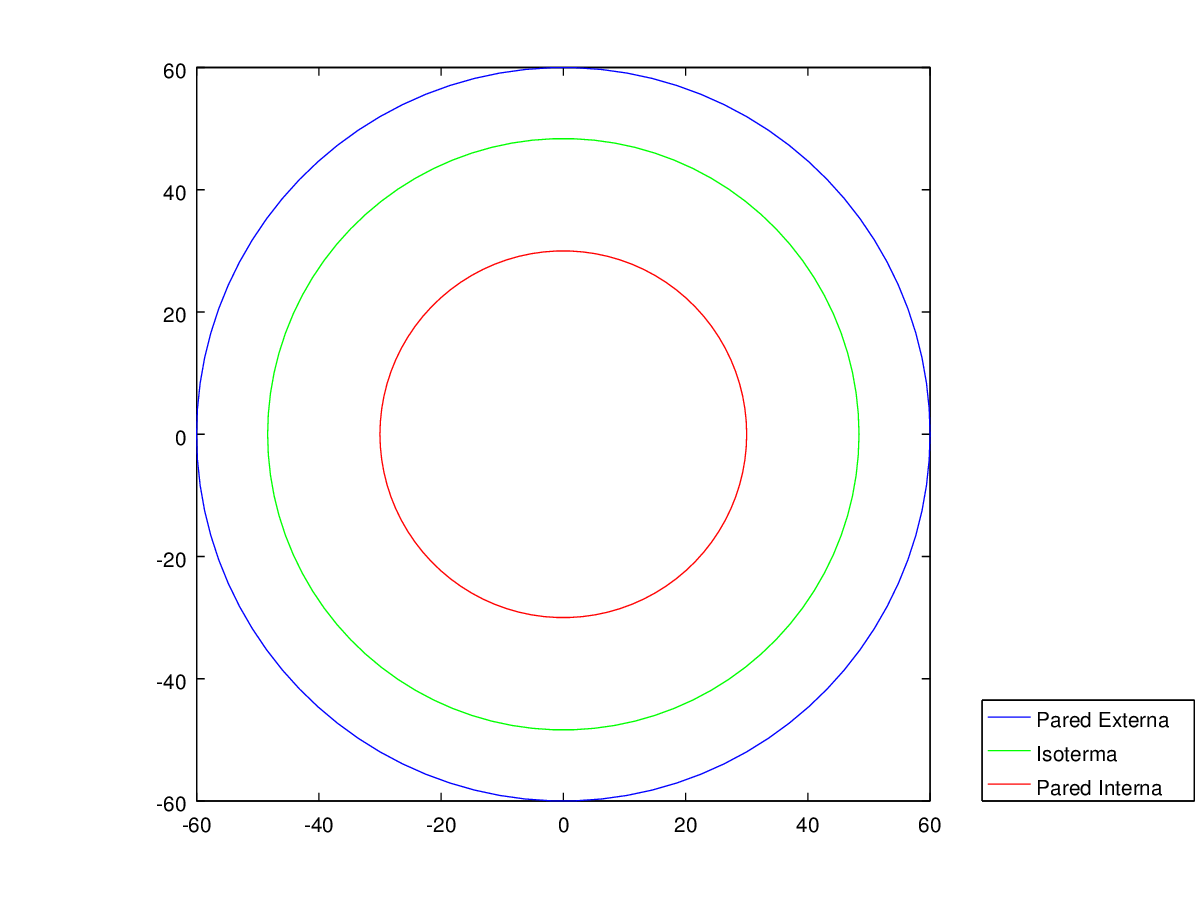
\includegraphics[height=5cm]{graficos/exp4/const/exp4-const-contraste-iso.png} \\
            {\small Temperaturas obtenidas} &
            {\small Posición estimada de la isoterma 500{\degree}C} \\
          \end{tabular}

        \end{center} \end{minipage}

        \vspace{1em}

        \begin{minipage}{\textwidth} \begin{center}

          \strong{Caso A} \vspace{1em}
               
          \begin{tabular}{ccc}
            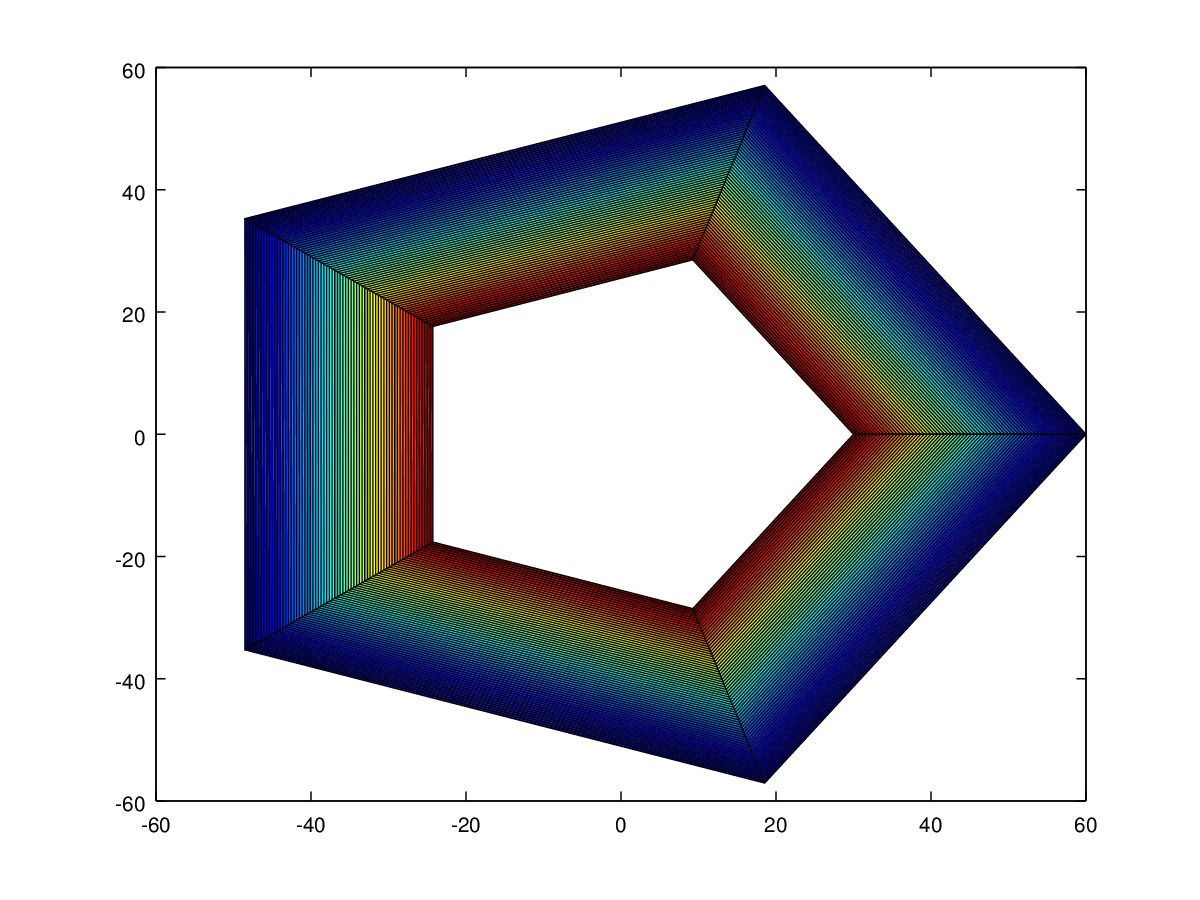
\includegraphics[width=4.5cm]{graficos/exp4/const/exp4-const-ang-5.png} &
            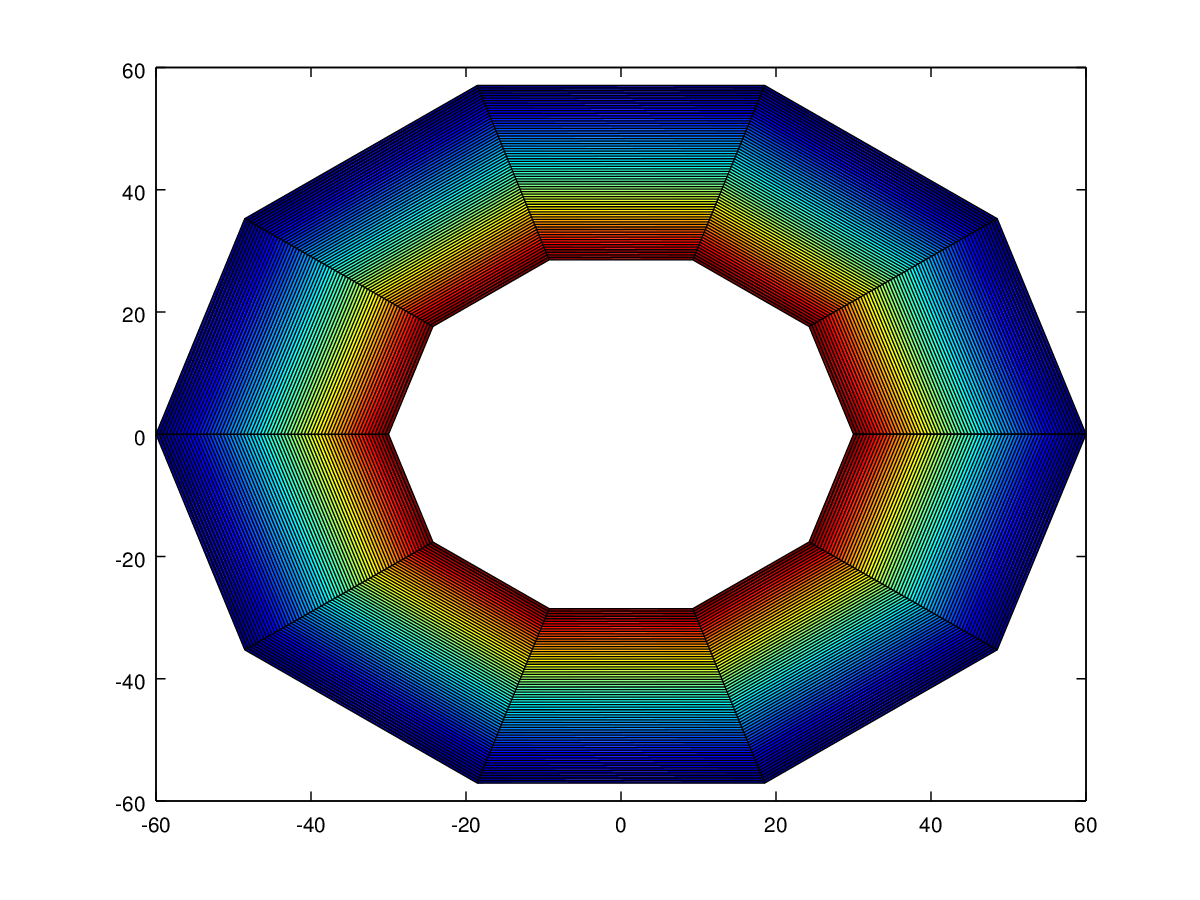
\includegraphics[width=4.5cm]{graficos/exp4/const/exp4-const-ang-10.png} &
            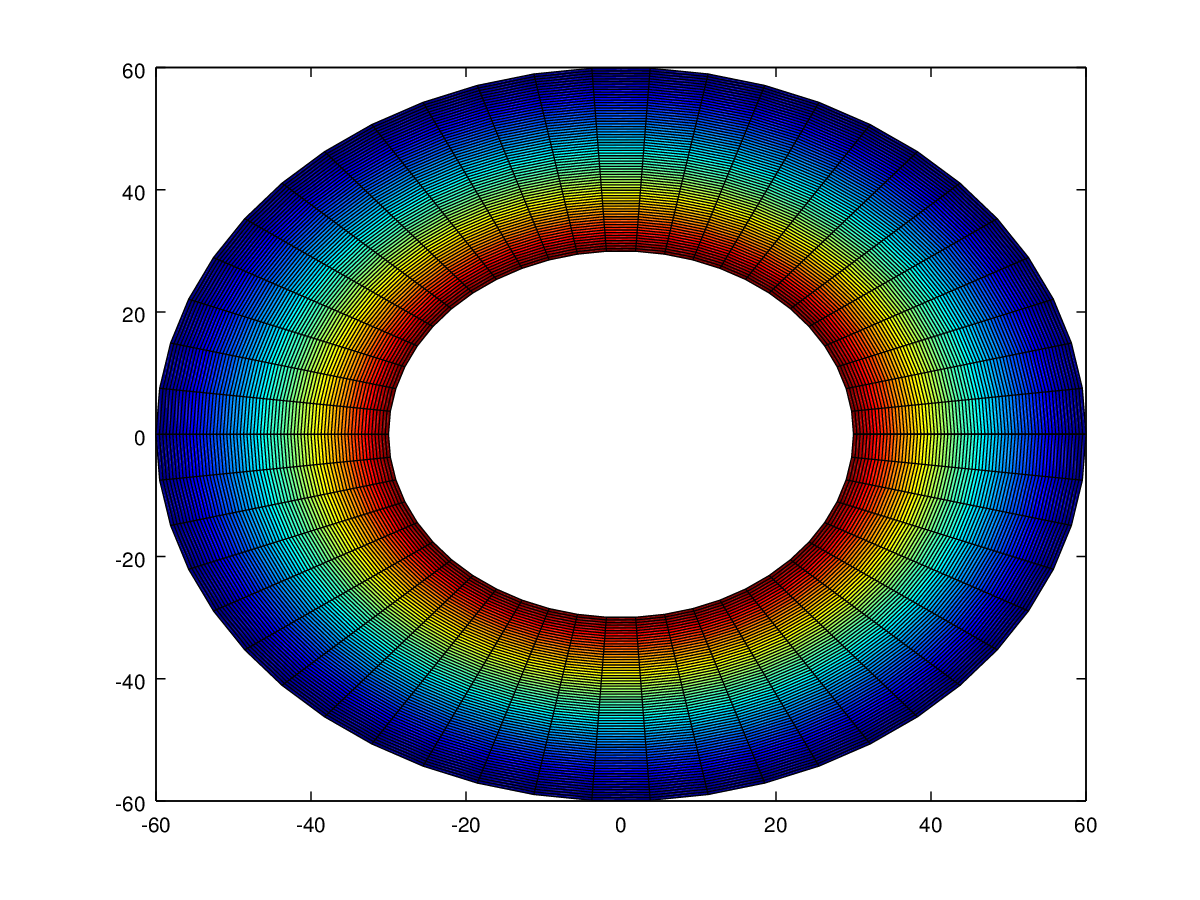
\includegraphics[width=4.5cm]{graficos/exp4/const/exp4-const-ang-50.png} \\
            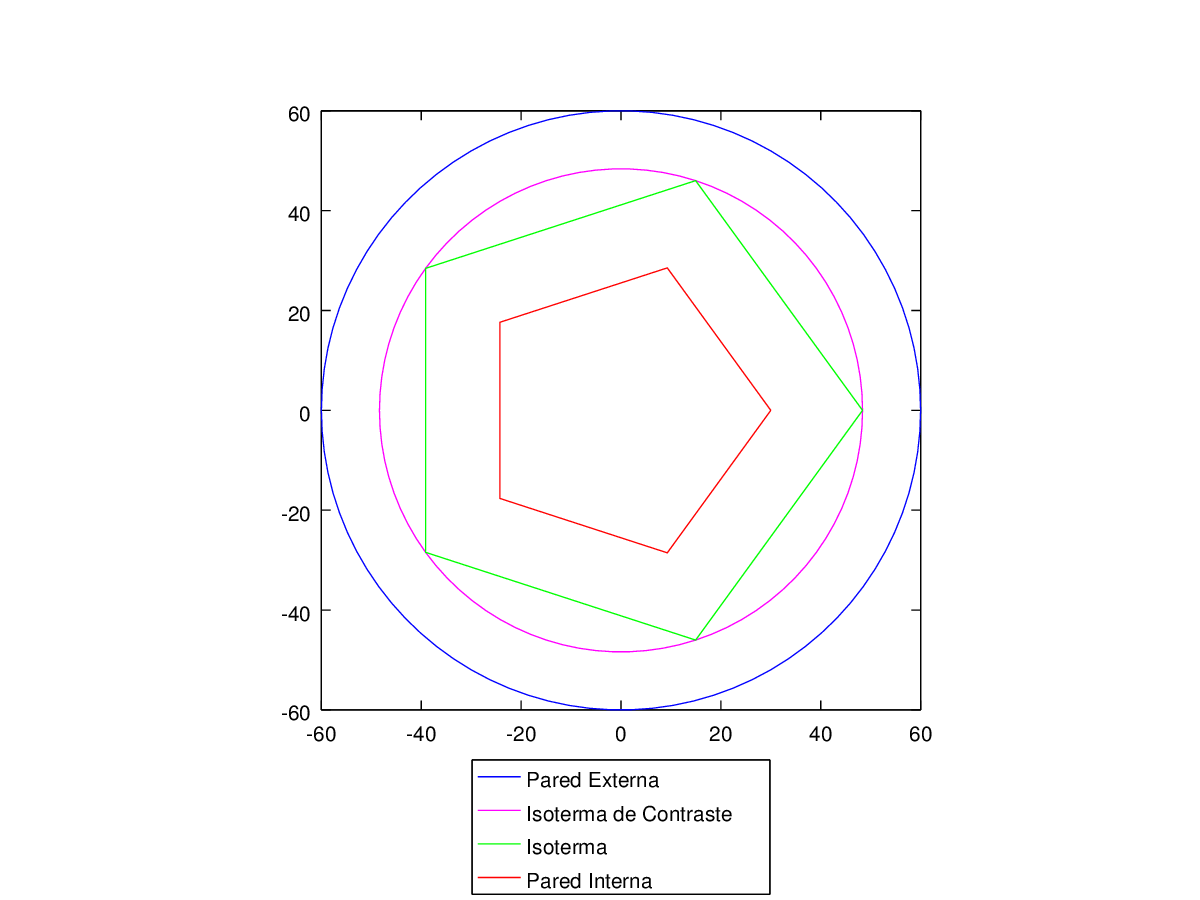
\includegraphics[width=5cm]{graficos/exp4/const/exp4-const-ang-5-iso.png} &
            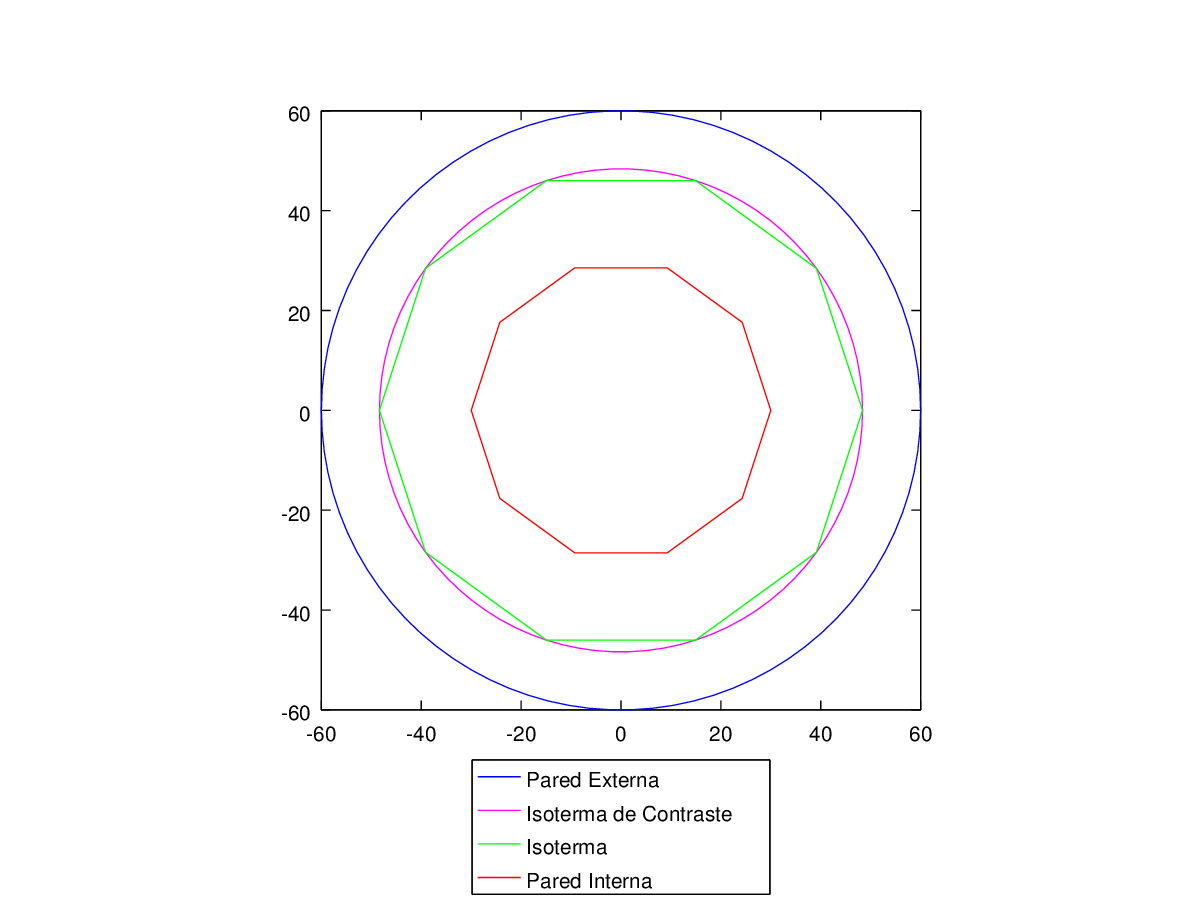
\includegraphics[width=5cm]{graficos/exp4/const/exp4-const-ang-10-iso.png} &
            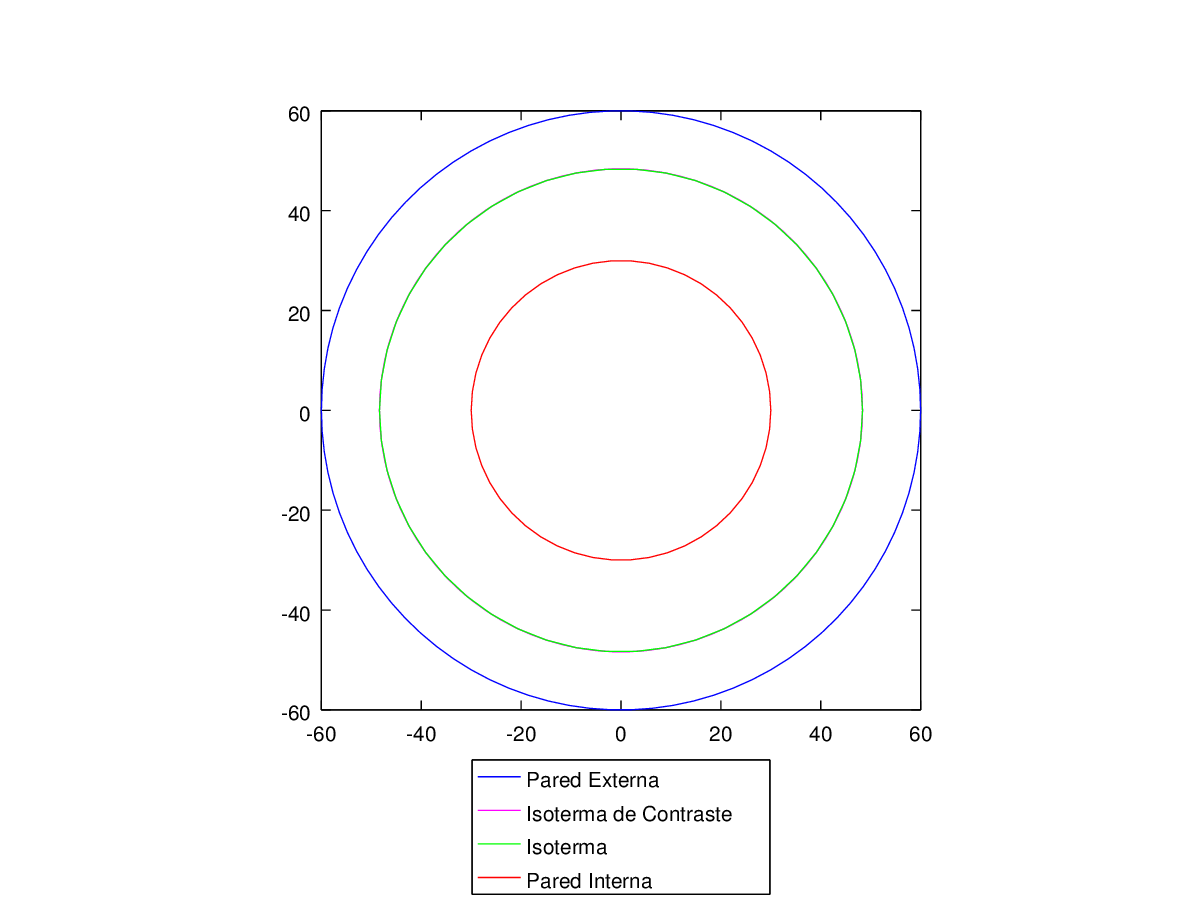
\includegraphics[width=5cm]{graficos/exp4/const/exp4-const-ang-50-iso.png} \\
            {\small $n = 5$} &
            {\small $n = 10$} &
            {\small $n = 50$} \\
          \end{tabular}

        \end{center} \end{minipage}

        \vspace{1em}

        \begin{minipage}{\textwidth} \begin{center}

          \strong{Caso B} \vspace{1em}
      
          \begin{tabular}{ccc}
            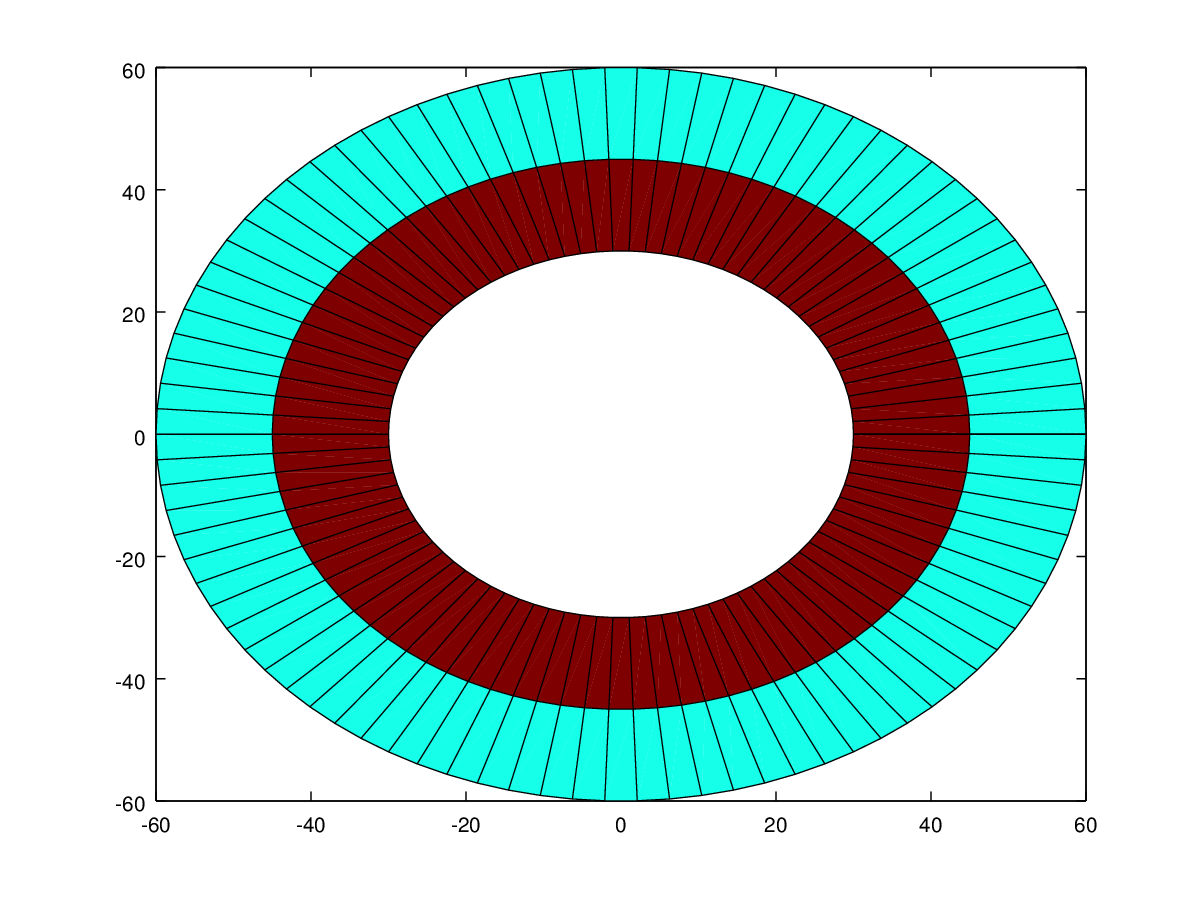
\includegraphics[width=4.5cm]{graficos/exp4/const/exp4-const-rad-3.png} &
            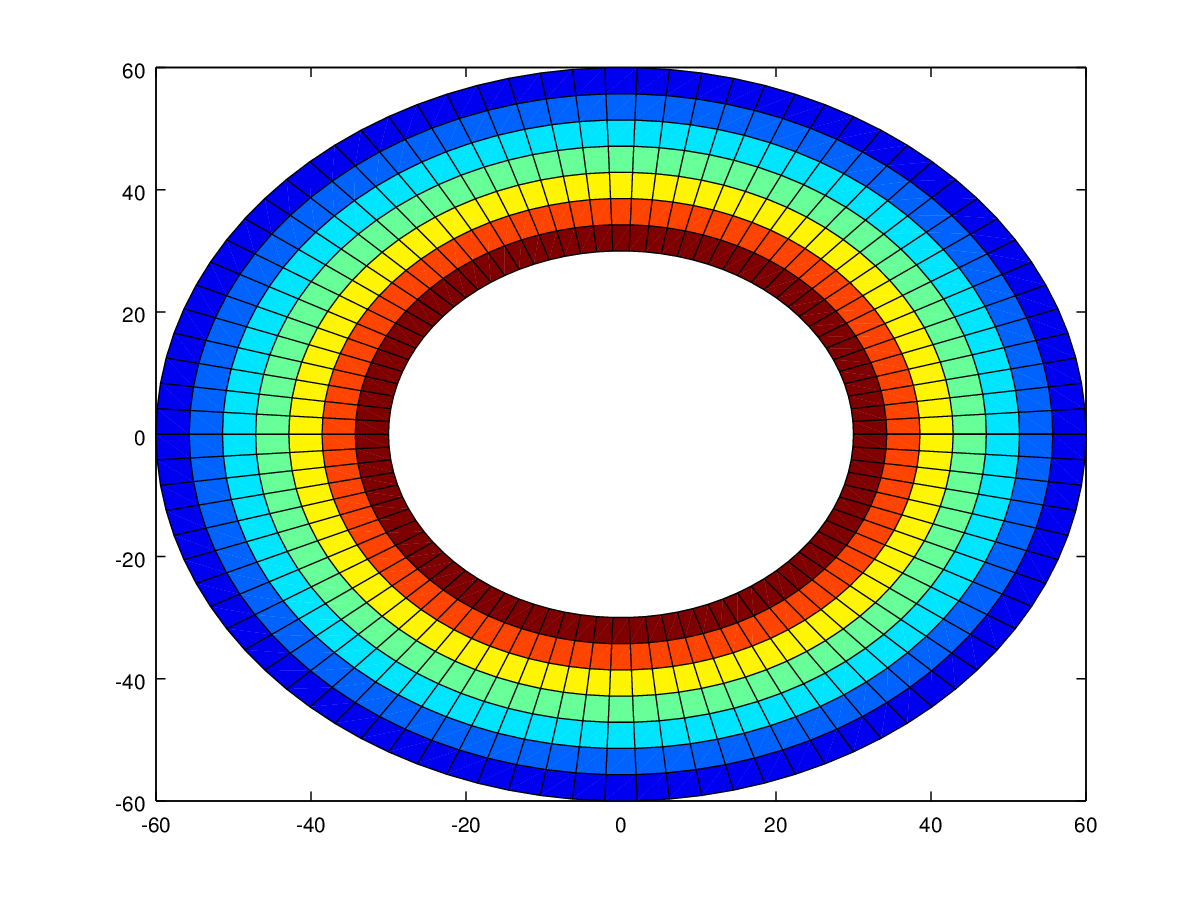
\includegraphics[width=4.5cm]{graficos/exp4/const/exp4-const-rad-8.png} &
            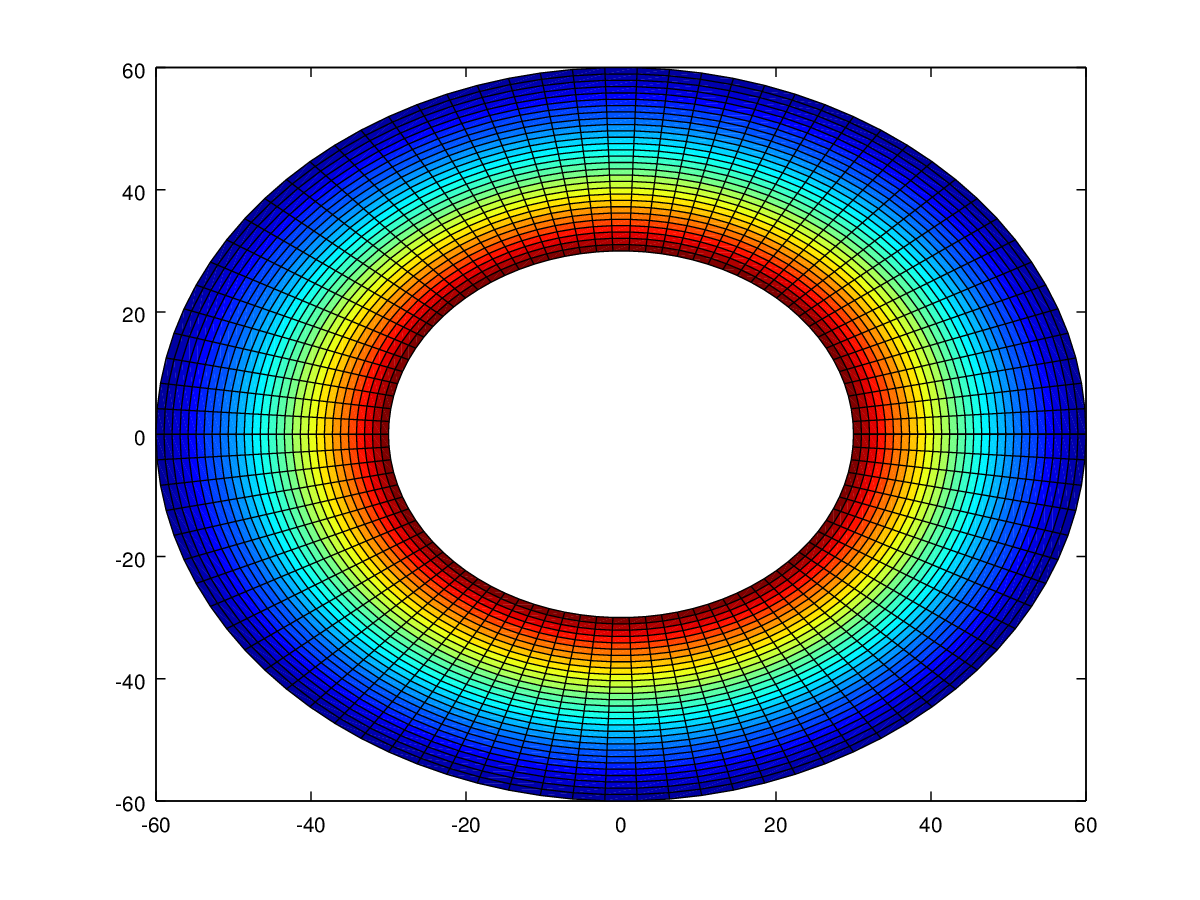
\includegraphics[width=4.5cm]{graficos/exp4/const/exp4-const-rad-30.png} \\
            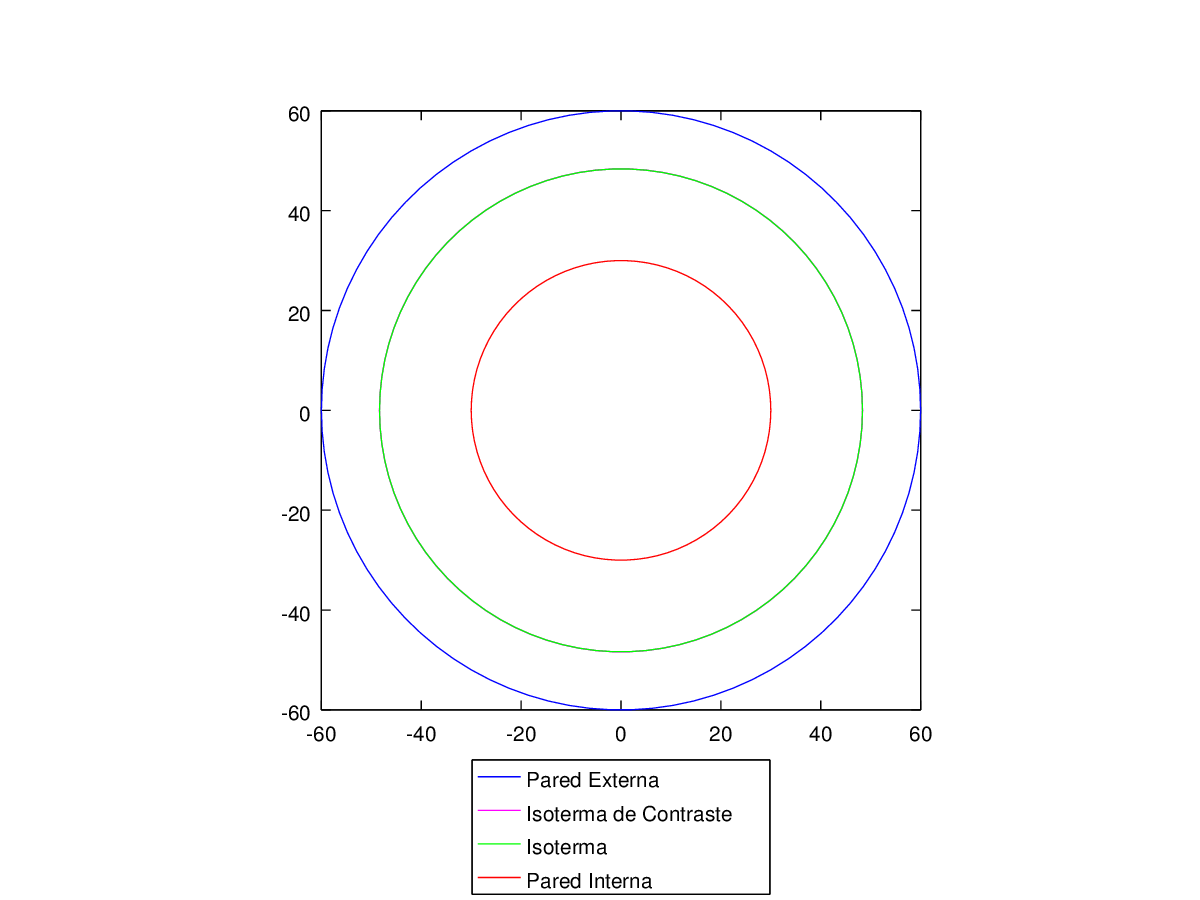
\includegraphics[width=5cm]{graficos/exp4/const/exp4-const-rad-3-iso.png} &
            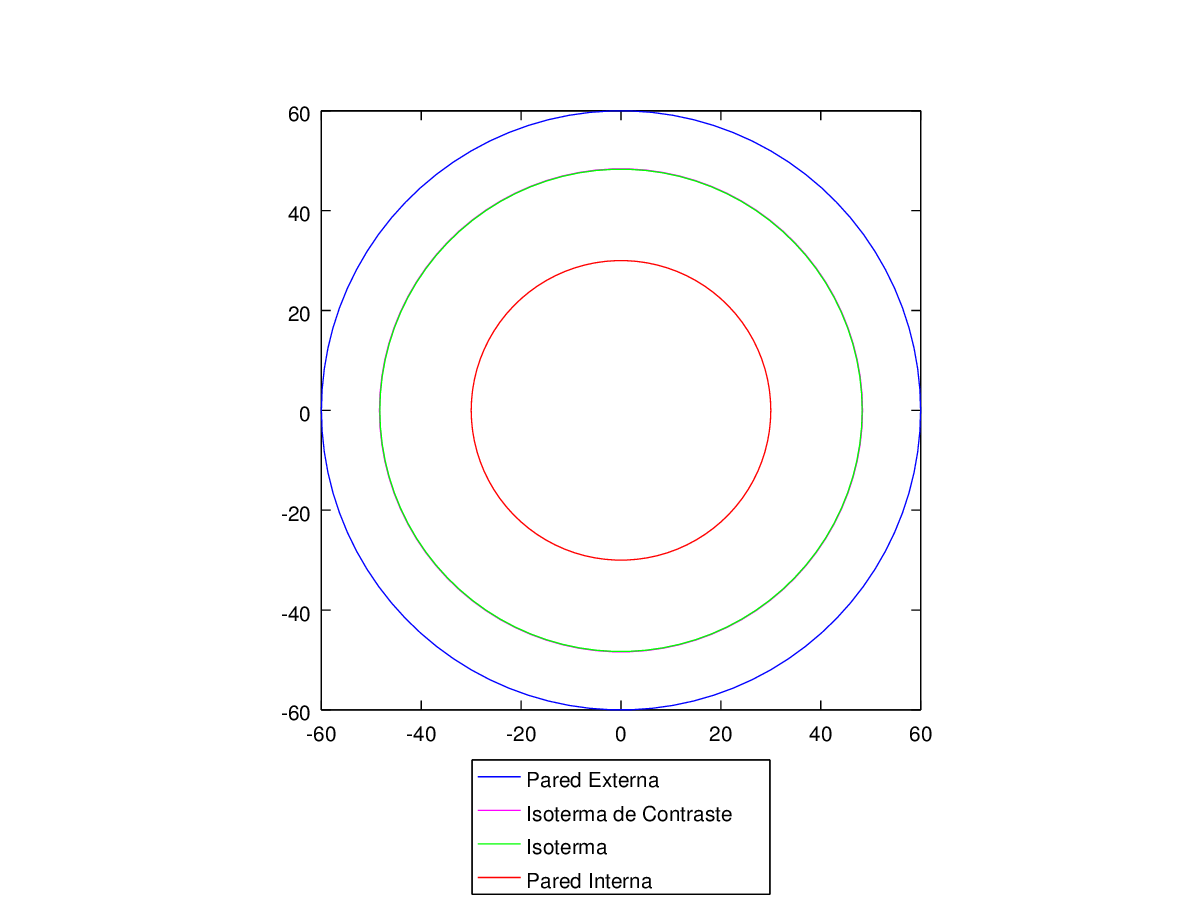
\includegraphics[width=5cm]{graficos/exp4/const/exp4-const-rad-8-iso.png} &
            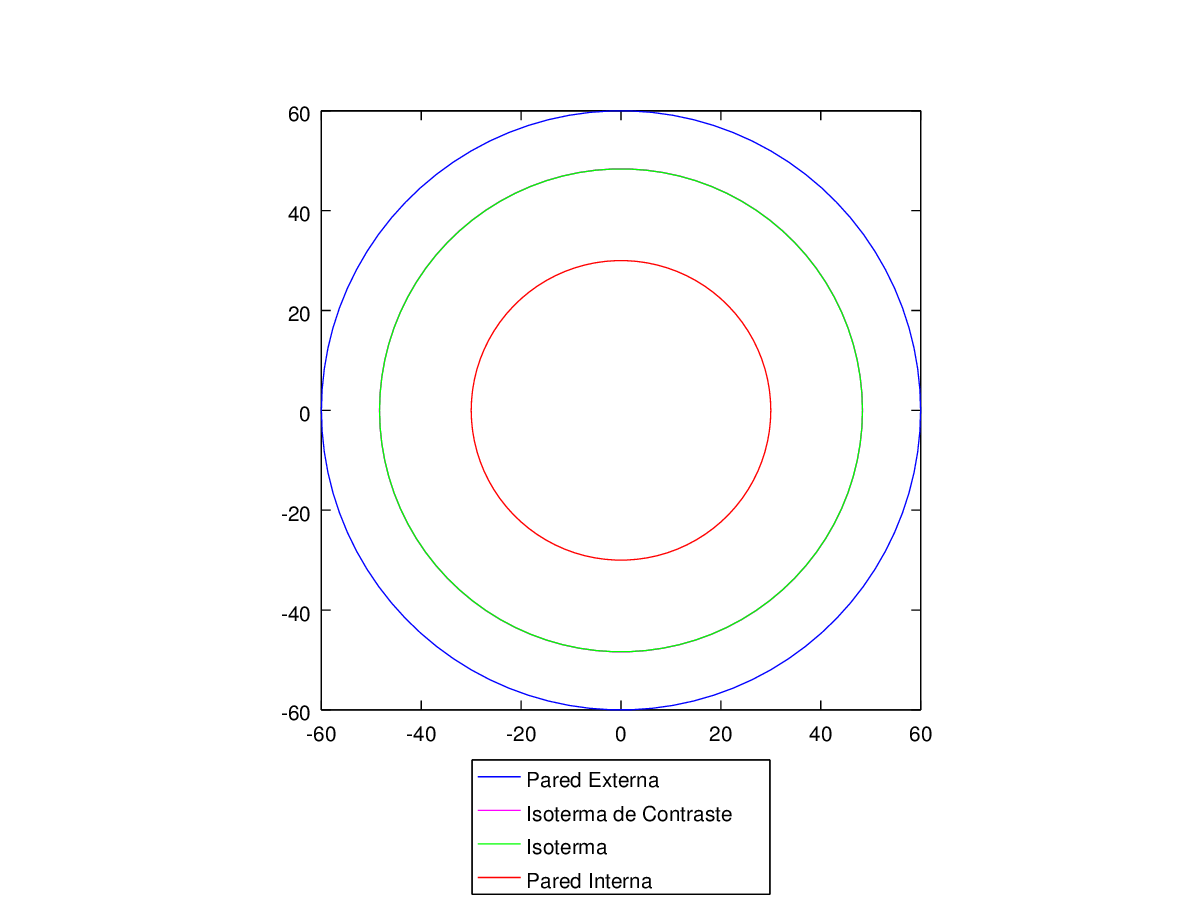
\includegraphics[width=5cm]{graficos/exp4/const/exp4-const-rad-30-iso.png} \\
            {\small $m+1 = 3$} &
            {\small $m+1 = 8$} &
            {\small $m+1 = 30$} \\
          \end{tabular}

        \end{center} \end{minipage}

        \vspace{1em}

        \begin{minipage}{\textwidth}

        (\textsc{ii}) \strong{Temperaturas variables}

        \begin{center}

          \strong{Caso de contraste} ($m + 1 = 70$ y $n = 90$)

          \begin{tabular}{cc}
            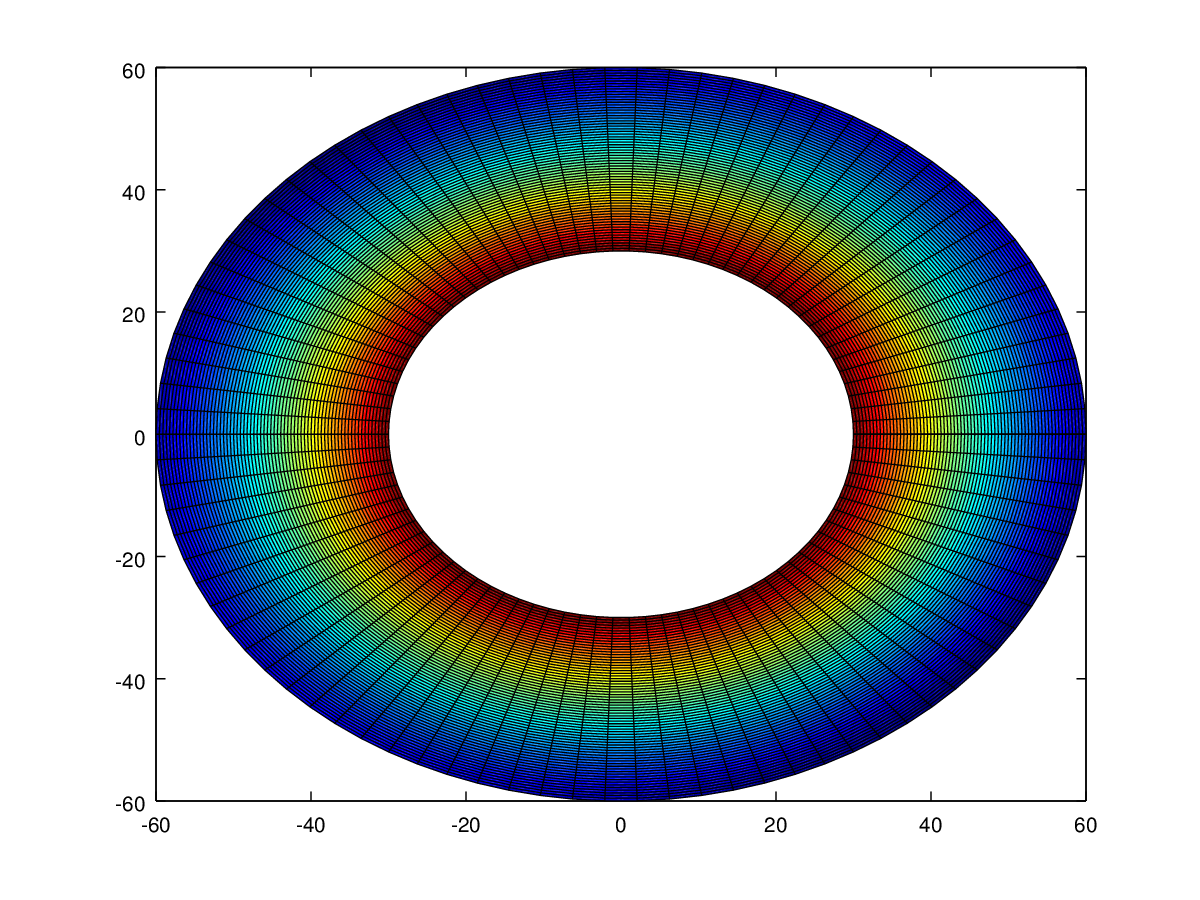
\includegraphics[height=5cm]{graficos/exp4/seno/exp4-seno-contraste.png} & 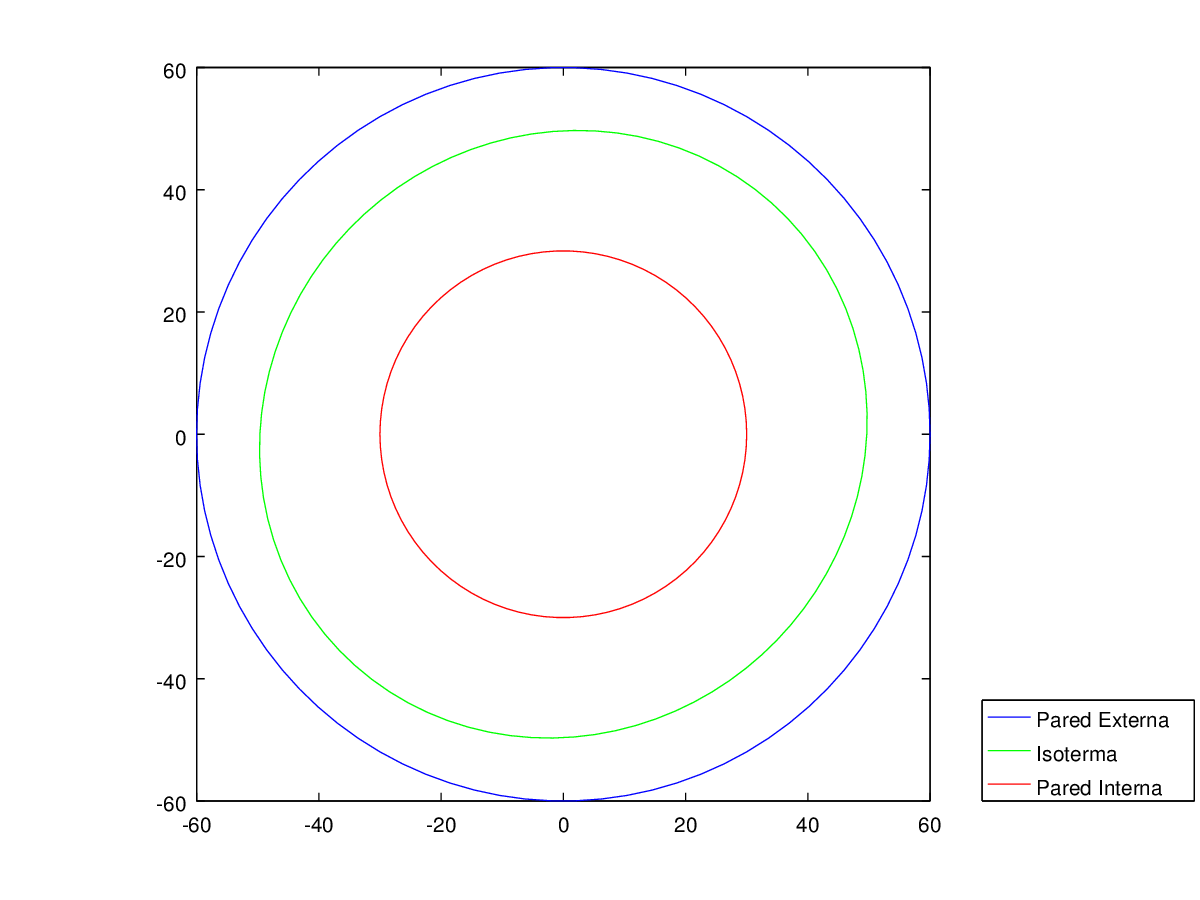
\includegraphics[height=5cm]{graficos/exp4/seno/exp4-seno-contraste-iso.png} \\
            {\small Temperaturas obtenidas} &
            {\small Posición estimada de la isoterma 500{\degree}C} \\
          \end{tabular}

        \end{center} \end{minipage}

        \vspace{1em}

        \begin{minipage}{\textwidth} \begin{center}

          \strong{Caso A} \vspace{1em}

          \begin{tabular}{ccc}
            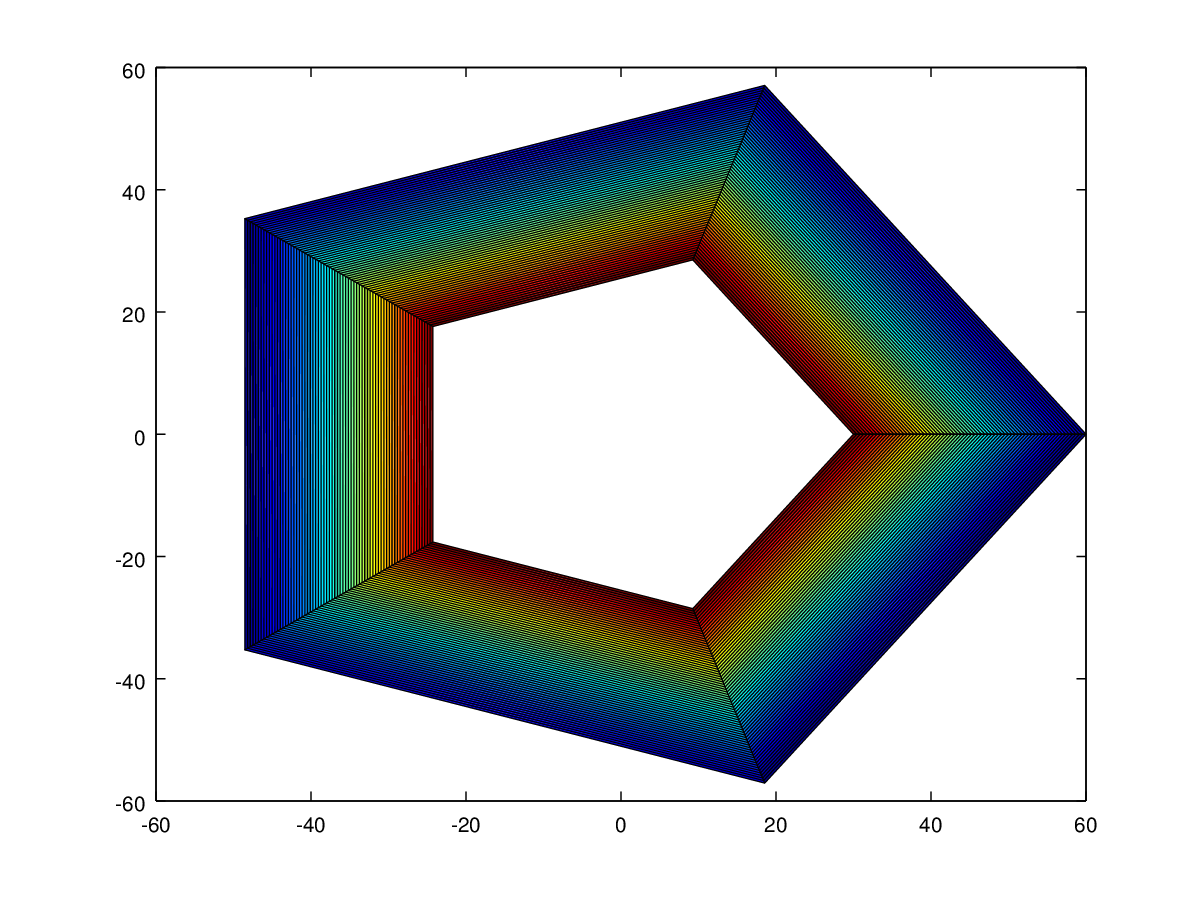
\includegraphics[width=4.5cm]{graficos/exp4/seno/exp4-seno-ang-5.png} &
            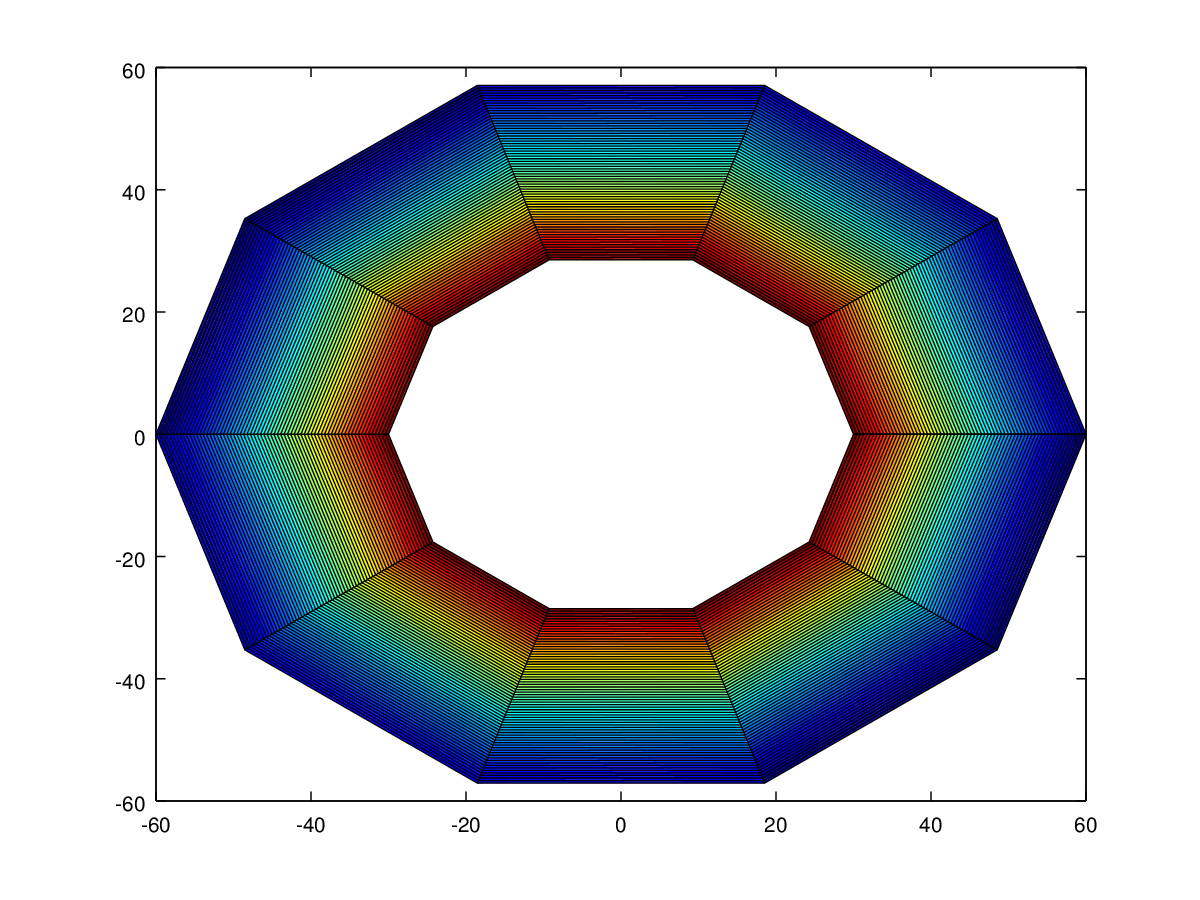
\includegraphics[width=4.5cm]{graficos/exp4/seno/exp4-seno-ang-10.png} &
            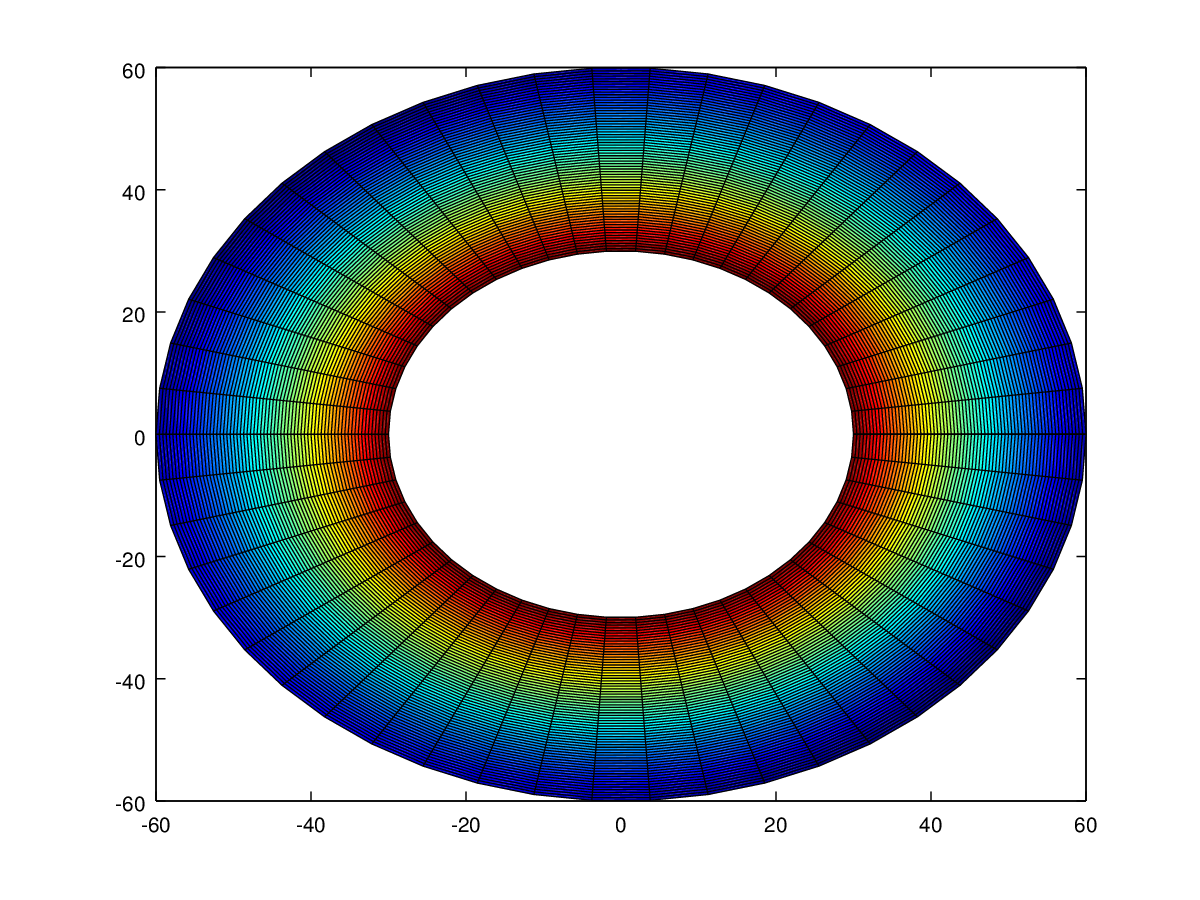
\includegraphics[width=4.5cm]{graficos/exp4/seno/exp4-seno-ang-50.png} \\
            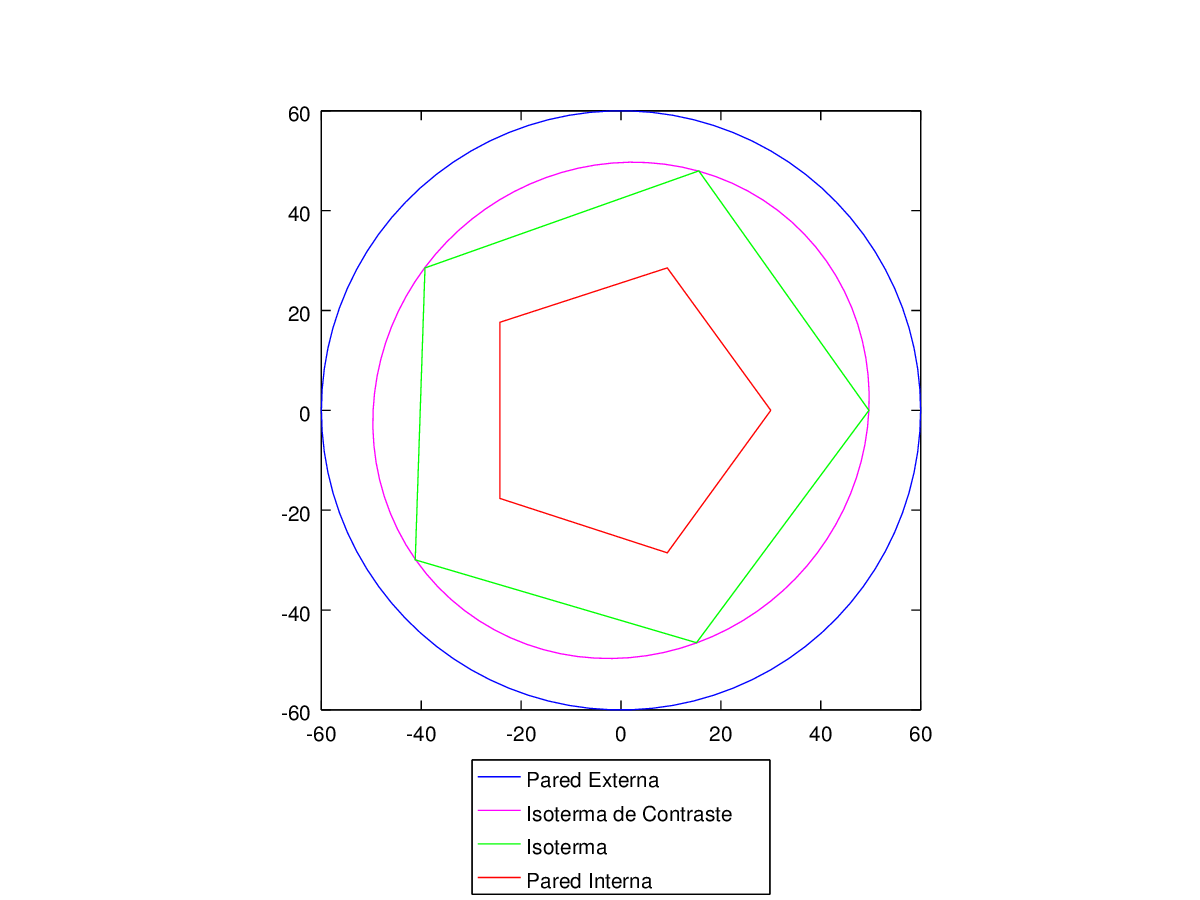
\includegraphics[width=5cm]{graficos/exp4/seno/exp4-seno-ang-5-iso.png} &
            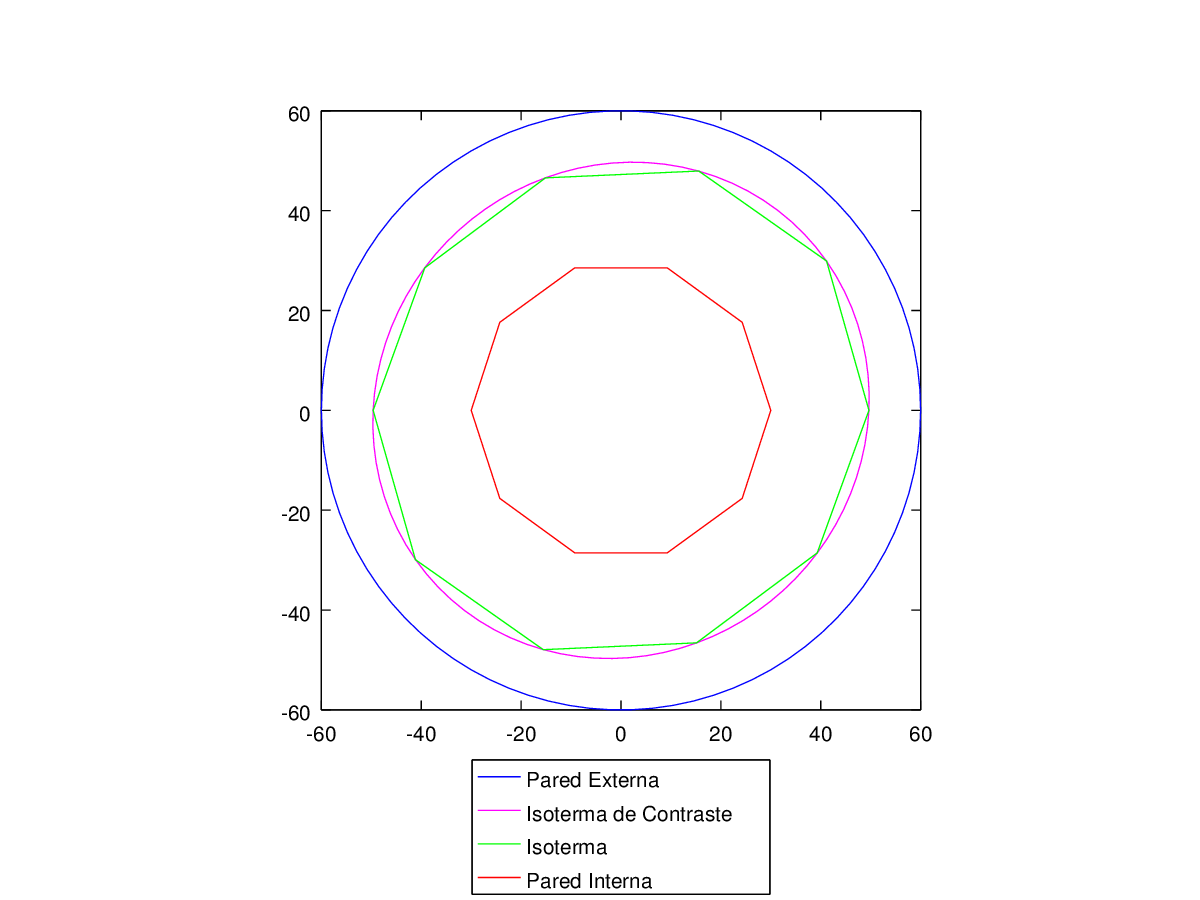
\includegraphics[width=5cm]{graficos/exp4/seno/exp4-seno-ang-10-iso.png} &
            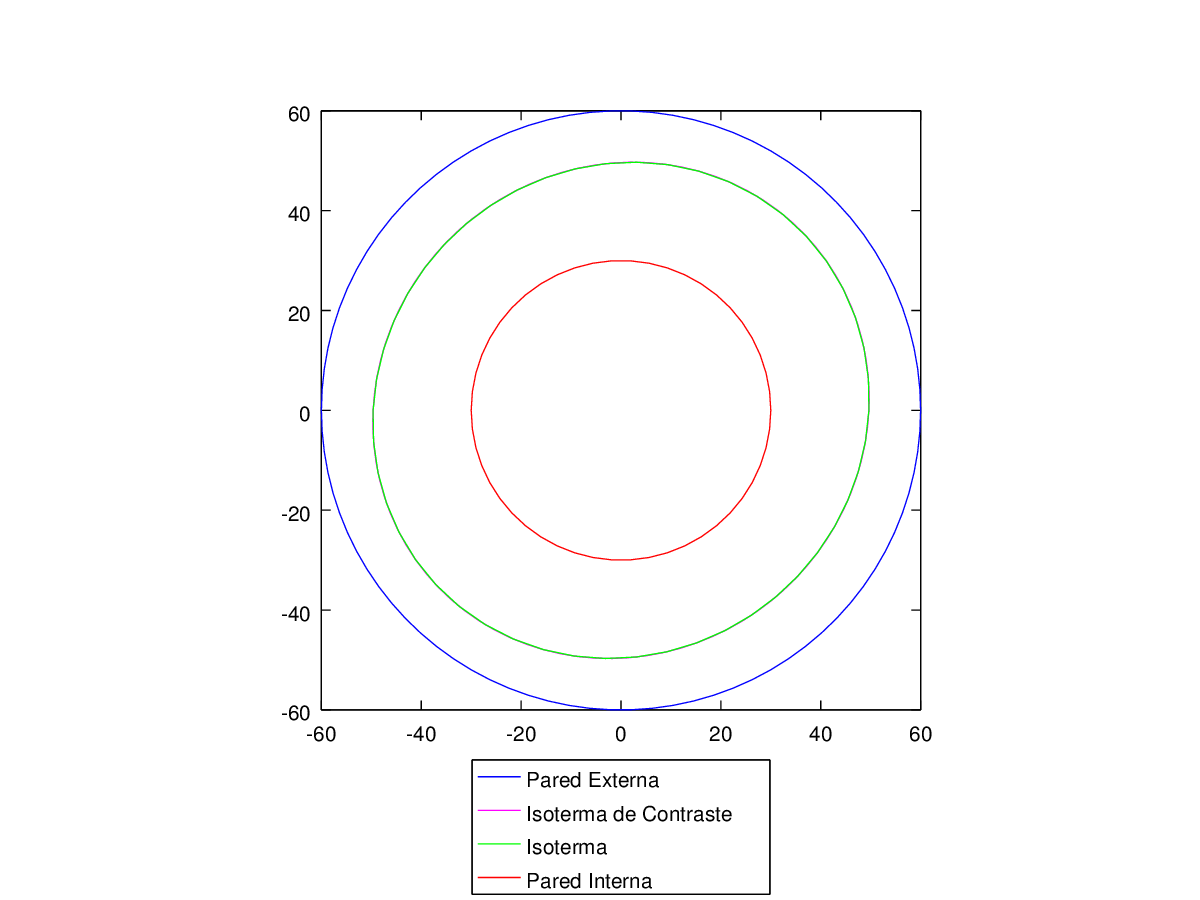
\includegraphics[width=5cm]{graficos/exp4/seno/exp4-seno-ang-50-iso.png} \\
            {\small $n = 5$} &
            {\small $n = 10$} &
            {\small $n = 50$} \\
          \end{tabular}

        \end{center} \end{minipage}

        \vspace{1em}

        \begin{minipage}{\textwidth} \begin{center}

          \strong{Caso B} \vspace{1em}

          \begin{tabular}{ccc}
            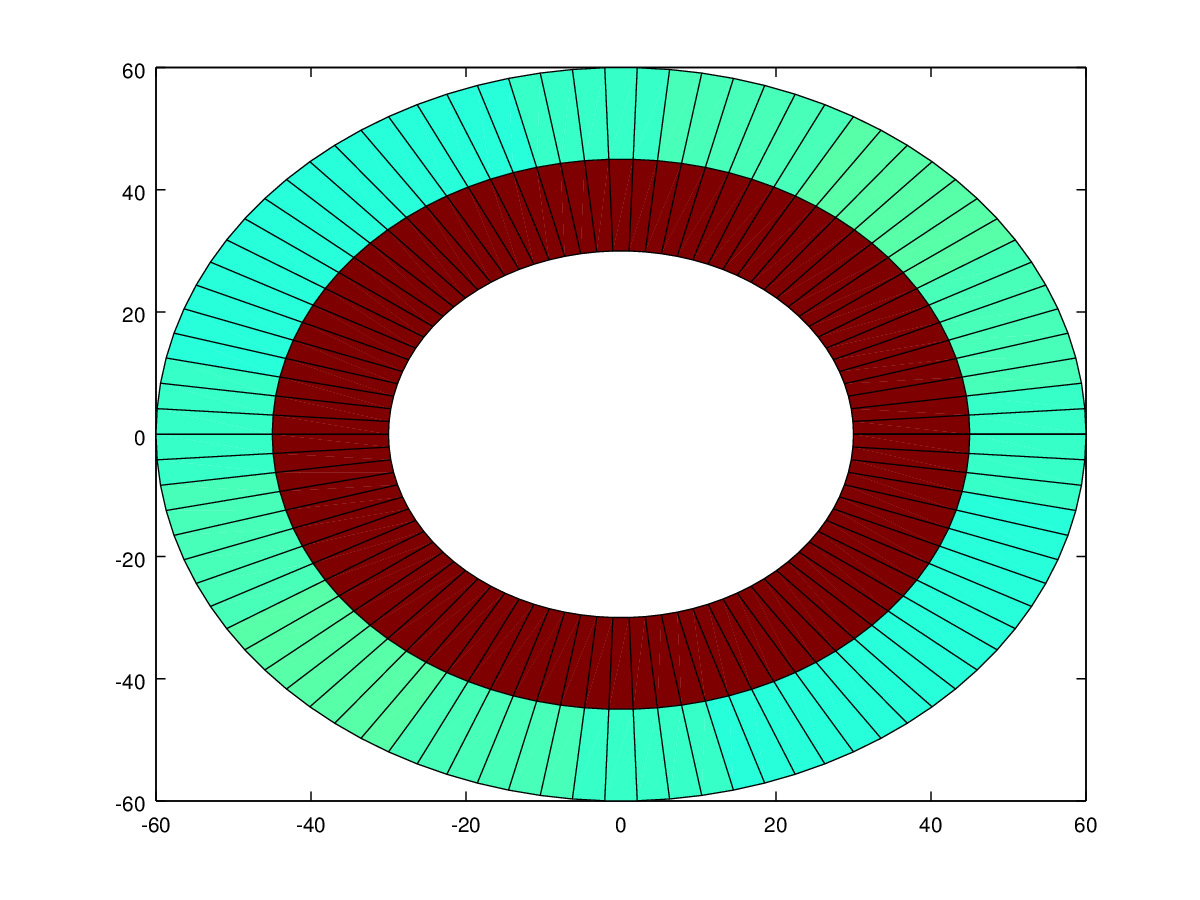
\includegraphics[width=4.5cm]{graficos/exp4/seno/exp4-seno-rad-3.png} &
            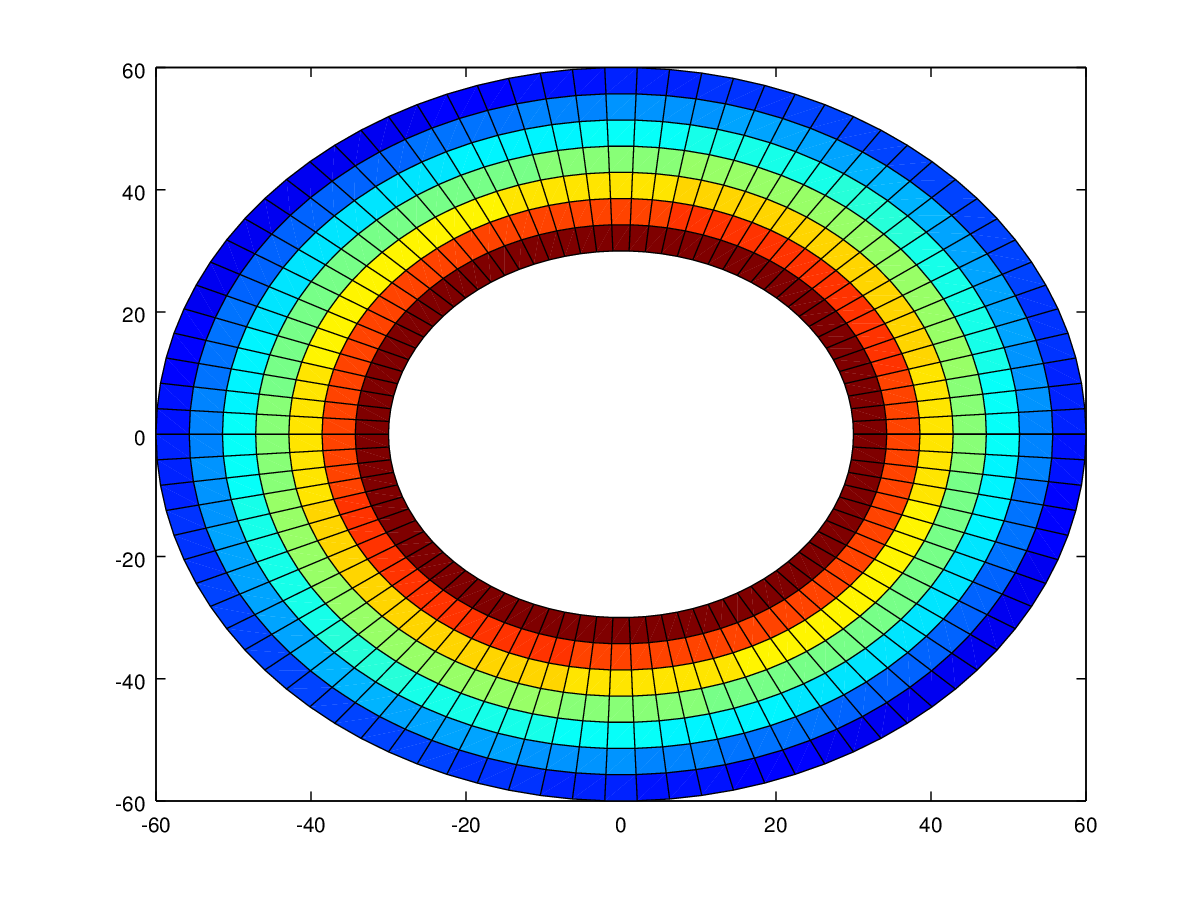
\includegraphics[width=4.5cm]{graficos/exp4/seno/exp4-seno-rad-8.png} &
            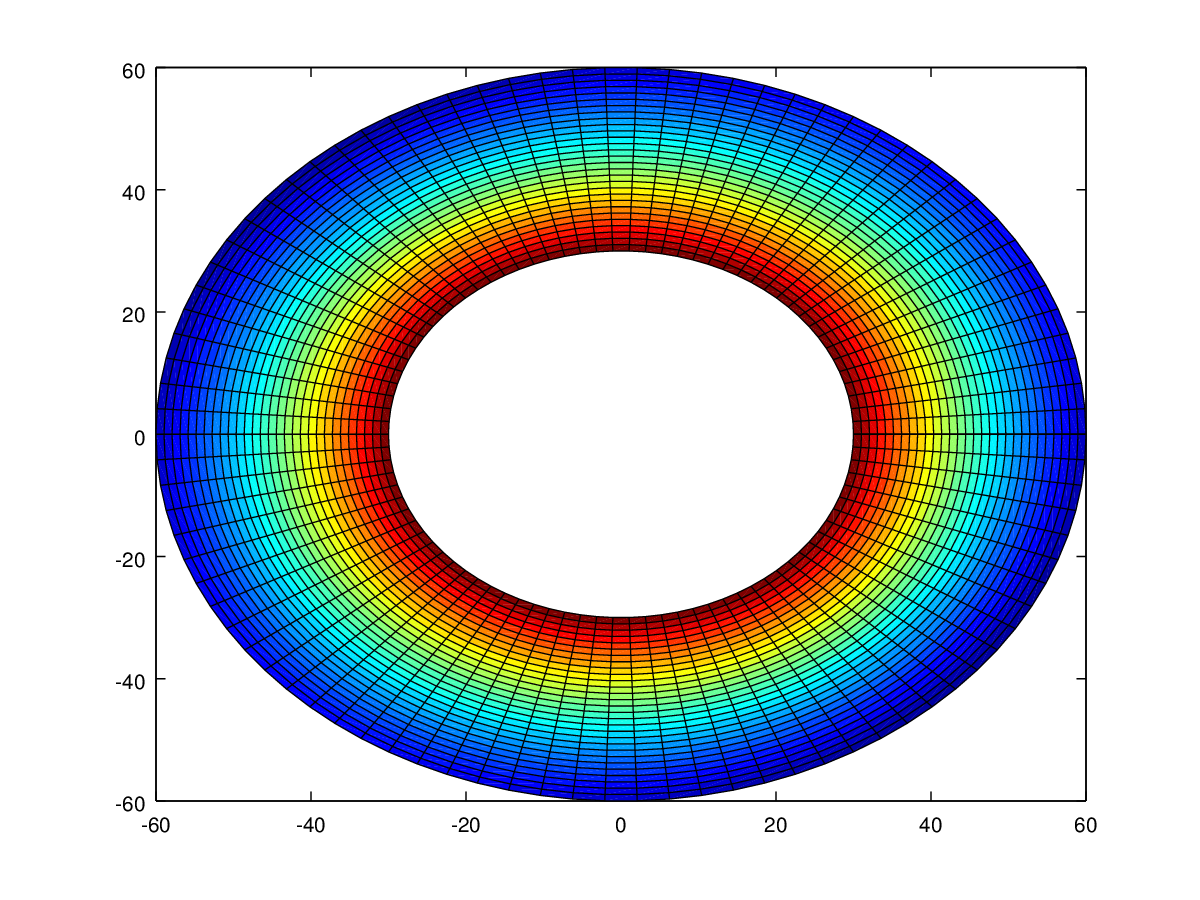
\includegraphics[width=4.5cm]{graficos/exp4/seno/exp4-seno-rad-30.png} \\
            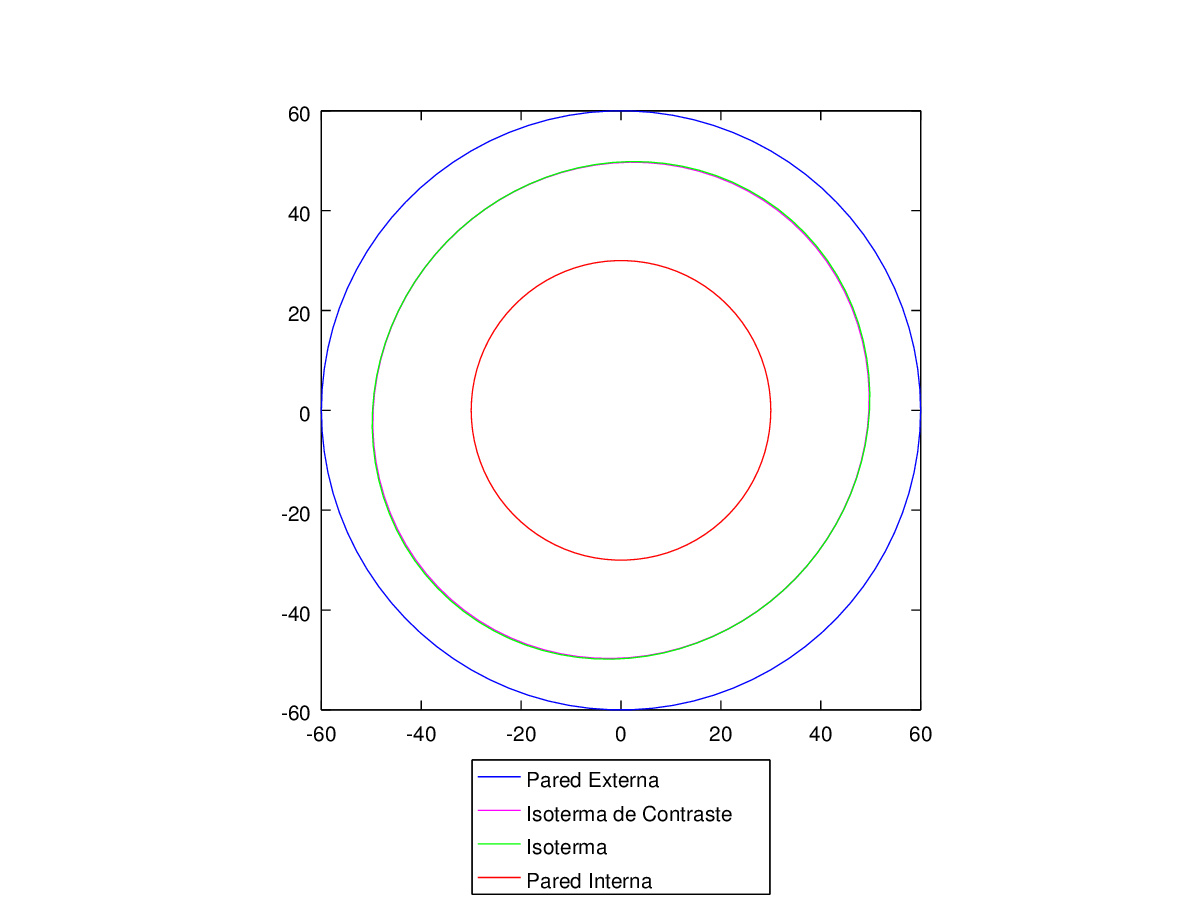
\includegraphics[width=5cm]{graficos/exp4/seno/exp4-seno-rad-3-iso.png} &
            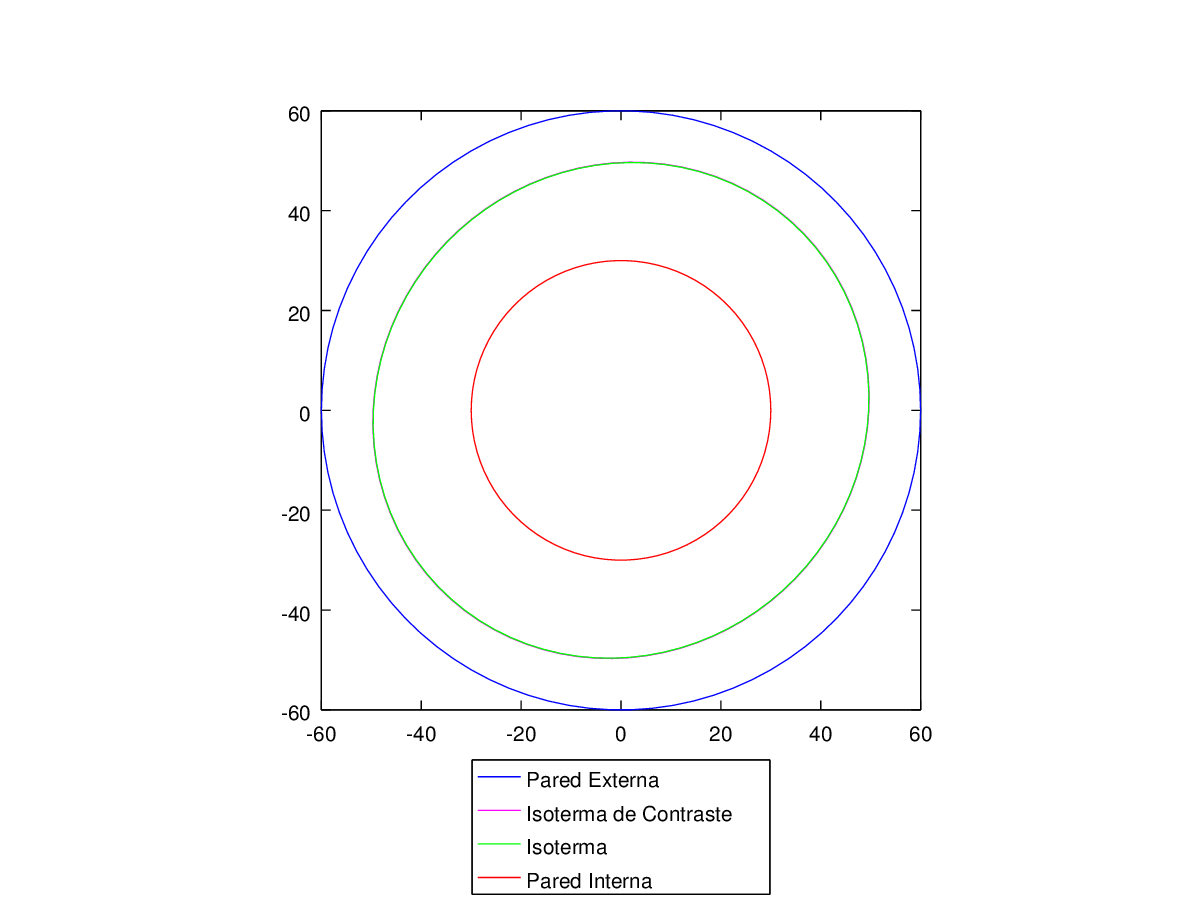
\includegraphics[width=5cm]{graficos/exp4/seno/exp4-seno-rad-8-iso.png} &
            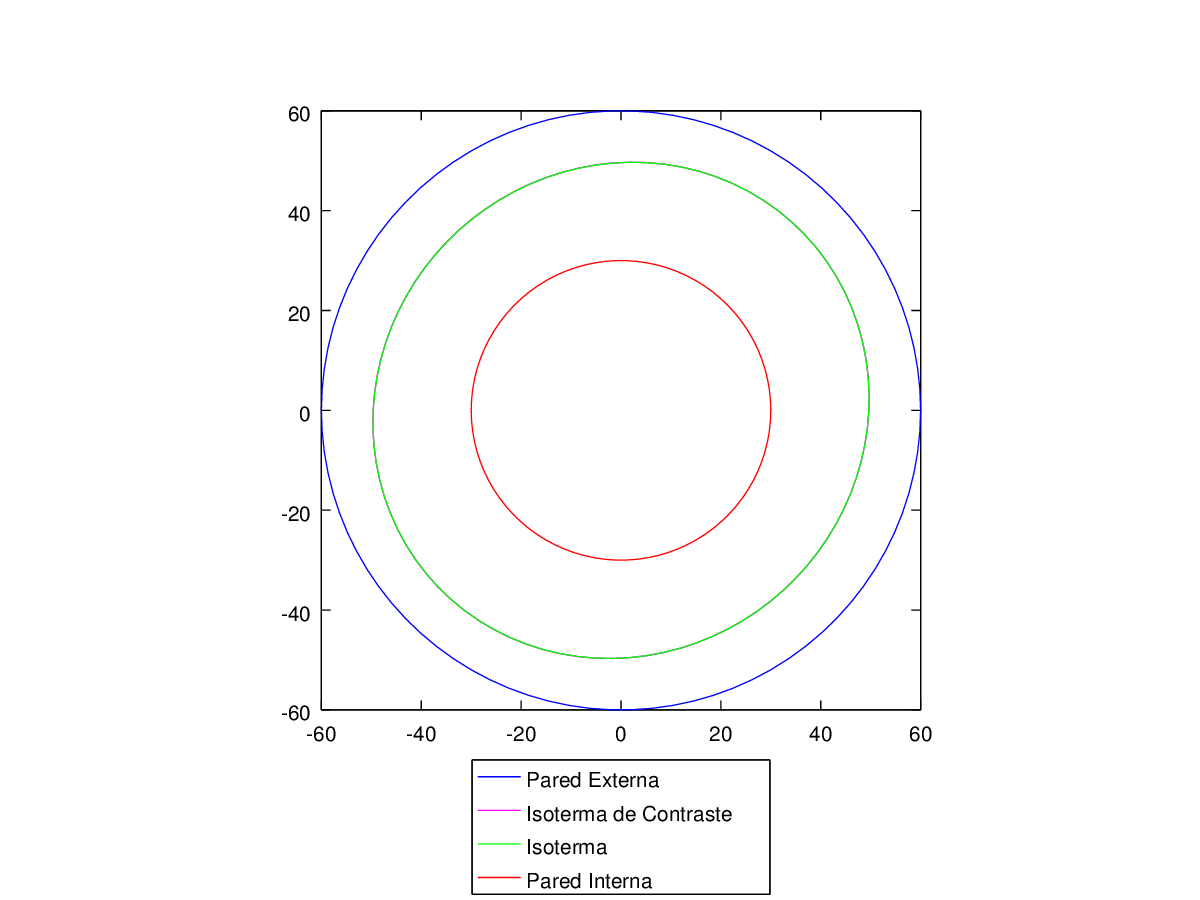
\includegraphics[width=5cm]{graficos/exp4/seno/exp4-seno-rad-30-iso.png} \\
            {\small $m+1 = 3$} &
            {\small $m+1 = 8$} &
            {\small $m+1 = 30$} \\
          \end{tabular}

        \end{center} \end{minipage}

      \subsubsection*{Discusión}
        Como se puede observar en los resultados, variar la granularidad con respecto a los ángulos no afecta al resultado de la posición de la isoterma. Ésta sigue siendo igual que la de contraste. Cuanto mayor cantidad de ángulos se tengan, más información podrá verse pero sin afectar el resultado total. En cambio, cuando modificamos la granularidad con respecto a los radios la isoterma calculada se aleja de la de contraste.

        Se deja abierta para experimentos futuros la posibilidad de observar qué tanto se modifica dependiendo de las temperaturas de la pared externa del horno. Para ello se podrían tomar valores de temperaturas externas mayores que 200{\degree}C y menores que 50{\degree}C a modo de análisis.

    \subsubsection{Experimento 5: Índice de peligrosidad según ancho de la pared}

      \subsubsection*{Presentación}
        Se busca estudiar la variación de la medida de peligrosidad con respecto al grosor de la pared del alto horno, sin modificar las temperaturas de la pared externa. Para ello se modificará el radio interno dejando constante el externo. Se realizará de esta manera ya que para lo que se quiere observar es indistinto cual de los dos variar. 

      \subsubsection*{Datos}
        Para este experimento se mantuvieron constantes los parámetros, $r_e = 90$, $m+1 = 30$, $n = 80$, $T_i = 1500$, $c = 500$, como así también la temperatura externa $T_e(\theta)$, para la cual se tomaron valores arbitrarios entre 50{\degree}C y 200{\degree}C. Se generaron instancias con los siguientes valores de $r_i$: $5, 10, 20, 40, 60, 80, 90$.  Se puede encontrar en los archivos adjuntos llamados \texttt{exp5-\{r\textsubscript{i}\}.in} la instancia pasada por parámetro.
     
      \subsubsection*{Hipótesis}
        La hipótesis de este experimento es que a medida que el grosor de la pared disminuye, el índice de peligrosidad aumenta, dado que al dejar las temperaturas constantes, la isoterma se encontrará cada vez más cerca de la pared externa. Esto sucede porque se acerca la pared interna (donde se encuentra la temperatura más alta del sistema) a la pared externa.
        
      \subsubsection*{Resultados}

        En el gráfico pueden observarse los valores obtenidos para el índice de peligrosidad en función de los diferentes valores de $r_i$.

          \begin{minipage}{\textwidth} \begin{center}
            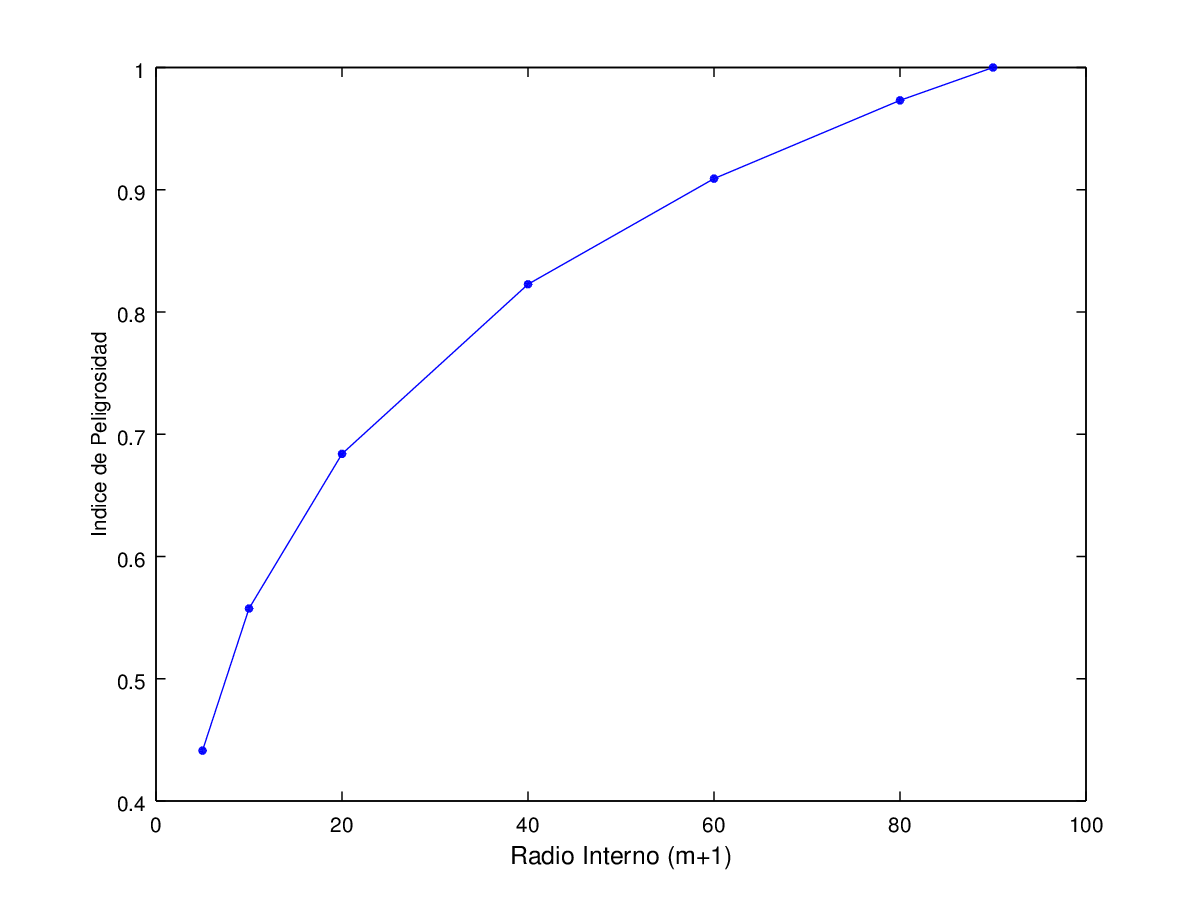
\includegraphics[width=11cm]{graficos/exp5/exp5.png} \\
            {\small Resultados arrojados por el experimento 5. Índice de peligrosidad en función del valor de $r_i$.}
          \end{center} \end{minipage}

      \subsubsection*{Discusión}
        En este experimento se puede ver que a medida que disminuye el grosor de la pared del alto horno, la isoterma se encuentra cada vez mas cerca de la pared externa. Dado que el índice de peligrosidad depende precisamente de la proximidad de la isoterma a la pared externa, cuando disminuye el grosor de la pared, el índice de peligrosidad aumenta, verificando así lo que se planteó en la hipótesis.
